% Generated by book/tools/notebook_to_tex.py. Do not edit by hand.

\chapter[한국어 BERT 보조 손실 (Korean Auxiliary Loss)]{한국어 BERT 보조 손실 (Korean Auxiliary Loss)}

\label{ch:18}

\markboth{한국어 BERT 보조 손실 (Korean Auxiliary Loss)}{한국어 BERT 보조 손실 (Korean Auxiliary Loss)}

\chaptermeta{18_ko_auxiliary/18_ko_auxiliary.ipynb}{https://colab.research.google.com/github/yoon-gu/neuqes-101/blob/master/18_ko_auxiliary/18_ko_auxiliary.ipynb}{한국어 다중 라벨 분류에 활성 라벨 개수 회귀 보조 헤드를 더해 결합 손실을 학습}



\index{1Korean BERT@Korean BERT}

\index{1KLUE BERT@KLUE-BERT}

\index{1klue bert base@klue/bert-base}

\index{1Auxiliary loss@Auxiliary loss}

\index{1multi task learning@multi-task learning}

\index{1combined loss@combined loss}

\index{1BCEWithLogitsLoss@BCEWithLogitsLoss}

\index{1MSELoss@MSELoss}

\index{1lambda@lambda}

\index{1AutoModel@AutoModel}

\index{1custom Trainer@custom Trainer}

\index{1compute loss@compute\_loss}

\index{1custom data collator@custom data collator}

\index{1auxiliary head@auxiliary head}

\index{1active label count@active label count}

\index{0한국어 BERT@한국어 BERT}

\index{0보조 손실@보조 손실}

\index{0멀티태스크 학습@멀티태스크 학습}

\index{0결합 손실@결합 손실}

\index{0보조 헤드@보조 헤드}

\index{0활성 라벨 수@활성 라벨 수}

\index{0커스텀 Trainer@커스텀 Trainer}

\index{0커스텀 데이터 콜레이터@커스텀 데이터 콜레이터}

\index{1lambda sweep@lambda sweep}

\index{1sweet spot@sweet spot}

\index{1lambda 0 05@lambda=0.05}

\index{0람다 스윕@람다 스윕}

\index{0약한 보조 신호@약한 보조 신호}

\index{1AutoModel from pretrained@AutoModel.from\_pretrained}

\index{1nn Module@nn.Module}

\index{1nn Linear@nn.Linear}

\index{1SequenceClassifierOutput@SequenceClassifierOutput}

\index{1Trainer compute loss@Trainer.compute\_loss}

\index{1remove unused columns False@remove\_unused\_columns=False}

\index{1lambda aux@lambda\_aux}

\index{1count head@count\_head}

\index{1Pearson correlation@Pearson correlation}

\index{1R2 score@R2 score}

\index{1RMSE@RMSE}

\index{1layer wise learning rate@layer-wise learning rate}

\index{0보조 라벨@보조 라벨}

\index{0활성 개수 회귀@활성 개수 회귀}

\index{0계층별 학습률@계층별 학습률}

\index{0보조 지표@보조 지표}

\index{0표현 공유@표현 공유}



\section{변화추적표}

\begin{booktable}{18장 변화추적표}{tab:ch18-01}
\begin{adjustbox}{max width=\textwidth}
\begin{tabular}{@{}lllllll@{}}
\toprule
Ch & 모델 & 토크나이저 & 데이터 & Output Head & Activation & Loss \\
\midrule

14 & DistilBERT + 보조 헤드 & WordPiece (영어) & Yelp + 항목 + 별점 & 메인(5) + 보조(1) & 메인 sigmoid + 보조 없음 & \texttt{BCE\ per-label\ +\ \$\textbackslash{}lambda\$·MSE} \\
16 & klue/bert-base & WordPiece (한국어) & KLUE-YNAT (뉴스 7분류) & \inlinecode{Linear(H,\ 7)} & softmax & \inlinecode{CrossEntropyLoss} \\
17 & klue/bert-base & 같음 & KLUE-YNAT 합성 multi-label & \inlinecode{Linear(H,\ 7)} & sigmoid (per-label) & \inlinecode{BCEWithLogitsLoss} (per-label) \\
\textbf{18 \(\leftarrow\) 여기} & klue/bert-base + \textbf{보조 헤드} & 같음 & KLUE-YNAT 합성 multi-label + \textbf{활성 개수} & \textbf{메인(7) + 보조(1)} & 메인 sigmoid + 보조 없음 & \textbf{\texttt{BCE\ per-label\ +\ \$\textbackslash{}lambda\$·MSE}} \\
19 (다음 Phase 3) & (없음) --- 토크나이저 학습 & \textbf{직접 학습한 워드레벨} & (코퍼스) & --- & --- & --- \\
\bottomrule
\end{tabular}
\end{adjustbox}
\end{booktable}

전체 장 표는 \href{https://github.com/yoon-gu/neuqes-101\#챕터별-변화추적표}{루트 README.md}를 참고하세요.



\section{변경점: \ref{ch:17}장 대비}

\begin{booktable}{18장 변경점 요약}{tab:ch18-02}
\begin{adjustbox}{max width=\textwidth}
\begin{tabular}{@{}lll@{}}
\toprule
축 & \ref{ch:17}장 (한국어 multi-label) & \ref{ch:18}장 (한국어 multi-label + auxiliary) \\
\midrule

Task (메인) & 7라벨 multi-label & (그대로) \\
\inlinecode{num\_labels} & 7 & (그대로) \\
메인 활성화 / loss & per-label sigmoid / BCE & (그대로) \\
\textbf{보조 head} & 없음 & \textbf{새로 추가}: \inlinecode{Linear(H,\ 1)} linear regressor \\
\textbf{보조 라벨} & 없음 & \textbf{새로 추가}: \inlinecode{n\_active} (활성 카테고리 \emph{개수}, 합성 과정에서 얻음 --- 1 또는 2) \\
\textbf{보조 loss} & --- & \textbf{\inlinecode{MSELoss}} (\ref{ch:09}·\ref{ch:14}장과 같은 식) \\
\textbf{결합 loss} & \inlinecode{outputs.loss} 자동 (BCE) & \textbf{\texttt{L\_main\ +\ \$\textbackslash{}lambda\$·L\_aux}} 직접 계산 \\
모델 구조 & \inlinecode{AutoModelForSequenceClassification} (자동 매핑) & \textbf{\inlinecode{AutoModel} 본체 + 메인 헤드 + 보조 헤드 직접 부착} (자동 매핑 X) \\
\inlinecode{Trainer.compute\_loss} & 자동 (오버라이드 X) & \textbf{오버라이드 필수} \\
데이터 콜레이터 & \inlinecode{DataCollatorWithPadding} 자동 & \textbf{커스텀} --- \inlinecode{n\_active} 도 같이 batching \\
학습 hyperparams & (epoch=2, lr=2e-5, bs=16, fp16) & (그대로) \\
\bottomrule
\end{tabular}
\end{adjustbox}
\end{booktable}

\begin{quote}
\textbf{변하는 축 --- Loss 축 끝 (한국어)}: 메인 task 와 모델 본체는 \emph{완전히 동일}, \emph{Loss 에 보조 항이 가중합으로 추가} 됩니다. \ref{ch:14}장 (영어) 와 같은 패턴을 한국어 데이터·모델로 재현. Phase 2 (한국어) 의 마지막 단계 --- 다음 Phase 3 에선 토크나이저 자체를 학습.
\end{quote}

\subsection{\texorpdfstring{왜 \emph{활성 라벨 개수} 가 좋은 보조 task 인가}{왜 활성 라벨 개수 가 좋은 보조 task 인가}}

합성 multi-label 데이터에서 \inlinecode{n\_active} 는 두 가지 좋은 보조 task 조건을 만족합니다:

\begin{enumerate}
\def\labelenumi{\arabic{enumi}.}
\tightlist
\item
  \textbf{공짜로 얻어짐} --- \inlinecode{make\_multilabel} 이 두 헤드라인을 결합할 때 활성 카테고리 개수가 자연히 부산물로 생김 (라벨링 비용 0). \ref{ch:14}장의 \emph{별점} 이 데이터에 \emph{원래} 있던 것과 비슷한 자연스러움.
\item
  \textbf{메인과 강한 상관} --- multi-label 정답 벡터 \(\mathbf{y}\) 와 그 \emph{합} \(\sum_k y_k = n_\text{active}\) 는 직접적으로 연결된 신호. 모델이 “이 헤드라인이 \emph{몇 개} 카테고리에 걸치는가” 를 잘 추정하면 “\emph{어느} 카테고리인가” 도 더 잘 맞힐 가능성 --- 두 task 가 같은 BERT 표현을 공유.
\end{enumerate}

\begin{quote}
\textbf{\ref{ch:14}장의 별점 vs \ref{ch:18}장의 활성 개수} --- \ref{ch:14}장 별점은 메인 (항목) 과 \emph{부분} 상관 (긍정 리뷰가 음식 라벨일 가능성 높음 정도). \ref{ch:18}장 활성 개수는 메인 (multi-label 벡터) 의 \emph{직접 함수} (합). 따라서 \ref{ch:18}장 이 \emph{원리적으로} auxiliary 효과가 더 명확하게 나타날 수 있는 셋업.
\end{quote}



\section{\texorpdfstring{손실 노트 --- Combined loss \texttt{L\ =\ L\_main\ +\ \$\textbackslash{}lambda\$\ ·\ L\_aux}}{손실 노트 --- Combined loss L = L\_main + \$\textbackslash lambda\$ · L\_aux}}

\begin{equation}
\label{eq:ch18-01}
L = \underbrace{\frac{1}{N \cdot K}\sum_{i,k}\text{BCE}(z_{i,k}^\text{main}, y_{i,k}^\text{main})}_{L_\text{main}: \text{카테고리 BCE per-label}} + \lambda \cdot \underbrace{\frac{1}{N}\sum_{i}(z_{i}^\text{aux} - n_{i}^\text{active})^2}_{L_\text{aux}: \text{활성 개수 MSE}}
\end{equation}

식~\eqref{eq:ch18-01}은 정답 라벨과 예측 확률 사이의 Binary Cross-Entropy를 정의합니다.

\begin{itemize}
\tightlist
\item
  \(z^\text{main} \in \mathbb{R}^7\) --- 카테고리 logit 7개, sigmoid 후 BCE per-label.
\item
  \(z^\text{aux} \in \mathbb{R}\) --- 활성 개수 회귀 logit (활성화 없음, 직접 MSE).
\item
  \(n^\text{active} \in \{1, 2\}\) --- 합성 시 두 헤드라인이 같은 카테고리면 1, 다르면 2 (이론상 1 또는 2 만 등장).
\item
  \(\lambda\) --- 보조 loss 가중치. 본문 기본값은 스윕에서 확인한 sweet spot 인 \textbf{0.05}입니다. 보조 MSE 가 메인 BCE 보다 \emph{크기 자체가 커서} \(\lambda\) 를 작게 잡아 균형을 맞춥니다.
\end{itemize}

\textbf{\(\lambda\) 스케일 감 잡기 --- 보조 MSE 의 \emph{크기} 부터}

활성 개수 정답은 1 또는 2 의 \emph{정수}. 학습 초기 보조 헤드 예측이 평균 1.5 근처면 MSE 는 약 \(0.25\), 무작위 예측이면 \(1-4\)까지 커질 수 있습니다. 메인 BCE 는 K=7 평균이라 학습 초반에도 \(0.3-0.7\) 수준입니다. 따라서 \emph{\(\lambda\)=1} 은 과하고, 부록 스윕에서는 \textbf{\(\lambda\)=0.05} 가 메인 F1 을 가장 끌어올렸습니다.

\begin{booktable}{18장 손실 노트 - Combined loss L = L\_main + \$\textbackslash lambda\$ · L\_aux 표}{tab:ch18-03}
\begin{adjustbox}{max width=\textwidth}
\begin{tabular}{@{}lllll@{}}
\toprule
\(\lambda\) & \(L_\text{main}\) (가정 0.45) & \(L_\text{aux}\) (가정 0.25) & \(L\) & 보조 비중 \\
\midrule

0.0 & 0.45 & (무시) & 0.45 & 0\% (= \ref{ch:17}장) \\
0.05 & 0.45 & 0.25 & 0.4625 & 2.7\% \(\leftarrow\) \textbf{본문 기본, sweet spot} \\
1.0 & 0.45 & 0.25 & 0.70 & 36\% (보조가 메인의 절반 이상 영향) \\
5.0 & 0.45 & 0.25 & 1.70 & 74\% (보조 우세 --- 메인 신호 묻힘) \\
\bottomrule
\end{tabular}
\end{adjustbox}
\end{booktable}

이 장에선 \textbf{\(\lambda\)=0.05} 로 학습하고 \(\lambda\)=0 baseline 과 비교합니다. 부록 \inlinecode{18\_ko\_auxiliary\_lambda\_sweep} 의 공정 seed 스윕에서 \(\lambda\)=0.05 가 micro/macro-F1 을 가장 끌어올리는 sweet spot 으로 확인됐기 때문입니다.

\begin{quote}
\textbf{Auxiliary 가 \emph{새 task} 가 아니라 \emph{loss 보조항} 인 이유} --- \inlinecode{n\_active} 회귀가 \emph{추론 시 결과} 로 필요한 게 아닙니다. 운영에선 메인 multi-label 만 쓰고 보조 헤드는 \emph{호출조차 하지 않음}. 학습 \emph{과정} 에서 BERT 본체를 더 일반적인 표상으로 끌고 가려는 \emph{정규화} 신호일 뿐입니다. 그래서 이 변화는 \emph{task 축} 이 아니라 \emph{loss 축} 에 보조 항을 더하는 변화로 분류됩니다 --- 보조 헤드는 task 를 신설하는 게 아니라 손실에 항을 추가할 뿐입니다.
\end{quote}



\section{토크나이저 노트}

\ref{ch:17}장과 \emph{완전히 동일} --- \inlinecode{klue/bert-base} 한국어 WordPiece, \inlinecode{max\_length=128}, 두 헤드라인을 \texttt{“\ {[}SEP{]}\ ”} 로 이어붙인 결합 텍스트. \textbf{토크나이저는 라벨에 무관} 하므로 보조 라벨 (\inlinecode{n\_active}) 추가로 인한 변화 없음.

\begin{previewBox}{미리보기}
\textbf{다음 장 (\ref{ch:19}장, Phase 3 시작)}: 토크나이저를 \emph{직접 학습}. 사전학습 모델에 의존하지 않고 코퍼스에서 워드레벨 어휘를 직접 만들어 봅니다 --- \ref{ch:01}장 부터 따라온 “토크나이저 시각” 의 클라이맥스. 본 장까지는 \emph{기성품 KLUE WordPiece 를 그대로 썼지만} 다음 장부터는 \emph{어휘 구성 자체가 학습 대상}.
\end{previewBox}



\Needspace{5\baselineskip}
\begin{lstlisting}
!pip install -q transformers datasets
\end{lstlisting}

\begin{codeRead}
\textbf{1행}의 \inlinecode{!pip install -q transform...}에서는 Colab 실행에 필요한 패키지를 설치합니다.
\end{codeRead}



\Needspace{11\baselineskip}
\begin{lstlisting}
import warnings
warnings.filterwarnings("ignore")

import numpy as np
import pandas as pd
import matplotlib.pyplot as plt
import seaborn as sns
import torch
import torch.nn as nn
import torch.nn.functional as F
from datasets import Dataset, load_dataset
from transformers import (
    AutoTokenizer, AutoModel,
    Trainer, TrainingArguments,
    DataCollatorWithPadding,
)
\end{lstlisting}

\noindent\emph{앞뒤 블록은 모두 필요한 라이브러리와 기본 설정을 준비하는 단계입니다. 길이를 나누어 같은 흐름을 단계별로 확인합니다.}

\Needspace{11\baselineskip}
\begin{lstlisting}[firstnumber=17]
from transformers.modeling_outputs import SequenceClassifierOutput
from sklearn.metrics import (
    precision_recall_fscore_support, classification_report,
    roc_auc_score, hamming_loss, mean_squared_error, r2_score,
)

import matplotlib.pyplot as plt, matplotlib.font_manager as fm, subprocess, os
_fp = "/usr/share/fonts/truetype/nanum/NanumGothic.ttf"
if not os.path.exists(_fp):
    subprocess.run(
        "apt-get -qq -y install fonts-nanum",
        shell=True,
    )
fm.fontManager.addfont(_fp)
plt.rcParams["font.family"] = "NanumGothic"
\end{lstlisting}

\noindent\emph{앞 블록은 필요한 라이브러리와 기본 설정을 준비하는 단계입니다. 이어지는 블록에서는 숫자 결과를 그림으로 확인하는 단계로 넘어갑니다.}

\Needspace{10\baselineskip}
\begin{lstlisting}[firstnumber=32]
plt.rcParams["axes.unicode_minus"] = False

if torch.cuda.is_available():
    DEVICE = "cuda"
elif getattr(torch.backends, "mps", None) is not None and torch.backends.mps.is_available():
    DEVICE = "mps"
else:
    DEVICE = "cpu"

\end{lstlisting}

\noindent\emph{앞 블록은 숫자 결과를 그림으로 확인하는 단계입니다. 이어지는 블록에서는 앞에서 만든 중간 값을 다음 계산으로 넘기는 단계로 넘어갑니다.}

\Needspace{11\baselineskip}
\begin{lstlisting}[firstnumber=41]
print(f"PyTorch:        {torch.__version__}")
print(f"CUDA available: {torch.cuda.is_available()}")
print(f"Device:         {DEVICE}")
if DEVICE == "cuda":
    print(
        f"GPU:             "
        f"{torch.cuda.get_device_name(0)}"
    )
elif DEVICE == "cpu":
    print(
        "Warning: CPU runtime — training will be very "
        "slow. Switch to T4 recommended."
    )
\end{lstlisting}

\begin{codeRead}
\inlinecode{numpy, pandas, matplotlib, PyTorch, datasets} 같은 주요 패키지를 불러옵니다.
\end{codeRead}

\noindent\textbf{출력.}
\begin{bookoutputbox}
PyTorch:        2.11.0+cu128
CUDA available: True
Device:         cuda
GPU:             Tesla T4
\end{bookoutputbox}
\par\vspace{0.9em}



\textbf{baseline VRAM} (CUDA 환경에서만 의미 있는 출력 --- Colab T4 기준):



\Needspace{5\baselineskip}
\begin{lstlisting}
!nvidia-smi
\end{lstlisting}

\begin{codeRead}
\textbf{1행}의 \inlinecode{!nvidia-smi}에서는 앞 단계에서 만든 값을 바탕으로 다음 계산을 수행합니다.
\end{codeRead}

\noindent\textbf{출력.}
\begin{bookoutputbox}
Wed Jun 24 21:40:30 2026
NVIDIA-SMI 580.82.07 Driver Version: 580.82.07 CUDA Version: 13.0
0 Tesla T4 Off | 00000000:00:04.0 Off | 0
N/A 35C P8 10W / 70W | 3MiB / 15360MiB | 0% Default
\end{bookoutputbox}
\par\vspace{0.9em}



\section{데이터 준비}

\ref{ch:17}장의 \inlinecode{make\_multilabel} 을 \emph{그대로} 가져옵니다. 함수 안에서 이미 \inlinecode{n\_active} (활성 라벨 개수) 컬럼이 만들어지고 있어 보조 라벨로 그대로 사용 가능 --- \emph{합성 과정의 자연스러운 부산물}.

\begin{booktable}{18장 데이터 준비 표}{tab:ch18-04}
\begin{adjustbox}{max width=\textwidth}
\begin{tabular}{@{}ll@{}}
\toprule
라벨 & 카테고리 \\
\midrule

0 & IT과학 \\
1 & 경제 \\
2 & 사회 \\
3 & 생활문화 \\
4 & 세계 \\
5 & 스포츠 \\
6 & 정치 \\
\bottomrule
\end{tabular}
\end{adjustbox}
\end{booktable}

\begin{quote}
\textbf{합성 규칙 (\ref{ch:17}장 동일)} --- 두 헤드라인 A, B 를 \texttt{“\ {[}SEP{]}\ ”} 로 연결, multi-hot 라벨에서 \(c_A, c_B\) 위치를 1 로. 우연히 \(c_A = c_B\) 면 활성 개수 1, 다르면 2. 7카테고리에서 무작위 결합이므로 \(P(c_A = c_B) = 1/7\) \(\to\) 평균 \inlinecode{n\_active} 약 \(2 \cdot 6/7 + 1 \cdot 1/7 \approx 1.86\).
\end{quote}



\Needspace{11\baselineskip}
\begin{lstlisting}
ds = load_dataset("klue/klue", "ynat")
print(f"splits: {list(ds.keys())}")
print(f"sizes: {[(k, len(v)) for k, v in ds.items()]}")

LABEL_NAMES = ds["train"].features["label"].names

_KO2EN = {"IT과학": "IT/Science", "경제": "Economy", "사회": "Society", "생활문화": "Life&Culture", "세계": "World", "스포츠": "Sports", "정치": "Politics"}
LABEL_NAMES_EN = [_KO2EN.get(n, n) for n in LABEL_NAMES]
K = len(LABEL_NAMES)
print(f"label names ({K}): {LABEL_NAMES}")

\end{lstlisting}

\noindent\emph{앞 블록은 데이터를 불러오고 학습에 맞는 형태로 정리하는 단계입니다. 이어지는 블록에서는 앞에서 만든 중간 값을 다음 계산으로 넘기는 단계로 넘어갑니다.}

\Needspace{9\baselineskip}
\begin{lstlisting}[firstnumber=12]
ds = ds.rename_column("title", "text")
print(f"\nfirst 2 raw samples:")
for ex in ds["train"].select(range(2)):
    print(
        f"  label={ex['label']} ({LABEL_NAMES_EN[ex['label']]:>12})  text="
        f"{ex['text']!r}"
    )
\end{lstlisting}

\noindent\textbf{출력.}
\begin{bookoutputbox}
splits: ['train', 'validation']
sizes: [('train', 45678), ('validation', 9107)]
label names (7): ['IT과학', '경제', '사회', '생활문화', '세계', '스포츠', '...

first 2 raw samples:
  label=3 (Life&Culture)  text='유튜브 내달 2일까지 크리에이터 지원 공간 운영'
  label=3 (Life&Culture)  text='어버이날 맑다가 흐려져…남부지방 옅은 황사'
\end{bookoutputbox}
\par\vspace{0.9em}



\subsection{\texorpdfstring{합성 함수 --- \ref{ch:17}장의 \inlinecode{make\_multilabel} 재사용}{합성 함수 --- \ref{ch:17}장의 make\_multilabel 재사용}}

\inlinecode{n\_active} (활성 개수) 컬럼이 합성 시 만들어집니다. \ref{ch:18}장의 보조 task 정답이 바로 이 값.



\Needspace{11\baselineskip}
\begin{lstlisting}
SEED = 42
N_TRAIN = 5000
N_EVAL  = 1000

def make_multilabel(source_split, n_samples, seed):
    '''single-label split 에서 두 샘플씩 결합해 multi-label 데이터셋 합성.

    - 2*n_samples 개 인덱스를 섞어 앞/뒤 절반을 짝으로 묶음
    - 텍스트는 " [SEP] " 로 이어붙임
    - multi-hot 라벨은 두 카테고리 위치를 1 로 (같은 카테고리면 1개만)
    - n_active 는 활성 카테고리 개수 (1 또는 2) — 18장 의 보조 task 정답
    '''
    rng = np.random.default_rng(seed)
    n_src = len(source_split)

\end{lstlisting}

\noindent\emph{앞뒤 블록은 모두 앞에서 만든 중간 값을 다음 계산으로 넘기는 단계입니다. 길이를 나누어 같은 흐름을 단계별로 확인합니다.}

\Needspace{11\baselineskip}
\begin{lstlisting}[firstnumber=16]
    idx = rng.integers(0, n_src, size=2 * n_samples).tolist()
    idx_a, idx_b = idx[:n_samples], idx[n_samples:]

    src_text = list(source_split["text"])
    src_label = list(source_split["label"])

    texts, multi_hots, active_counts = [], [], []
    for a, b in zip(idx_a, idx_b):
        ca, cb = int(src_label[a]), int(src_label[b])
        combined = f"{src_text[a]} [SEP] {src_text[b]}"
        mh = [0.0] * K
        mh[ca] = 1.0
        mh[cb] = 1.0
        texts.append(combined)
        multi_hots.append(mh)
        active_counts.append(int(sum(mh)))
\end{lstlisting}

\noindent\emph{앞뒤 블록은 모두 앞에서 만든 중간 값을 다음 계산으로 넘기는 단계입니다. 길이를 나누어 같은 흐름을 단계별로 확인합니다.}

\Needspace{11\baselineskip}
\begin{lstlisting}[firstnumber=32]
    return Dataset.from_dict({
        "text": texts,
        "multi_hot": multi_hots,
        "n_active": active_counts,
    })

train_full = make_multilabel(
    ds["train"],
    N_TRAIN,
    seed=SEED,
)
eval_full  = make_multilabel(
    ds["validation"],
    N_EVAL,
    seed=SEED + 1,
)
\end{lstlisting}

\noindent\emph{앞뒤 블록은 모두 앞에서 만든 중간 값을 다음 계산으로 넘기는 단계입니다. 길이를 나누어 같은 흐름을 단계별로 확인합니다.}

\Needspace{11\baselineskip}
\begin{lstlisting}[firstnumber=48]
print(f"synthetic train: {len(train_full)}")
print(f"synthetic eval:  {len(eval_full)}")
print(f"\nFirst synthetic sample:")
print(f"  text:      {train_full[0]['text']}")
print(f"  multi_hot: {train_full[0]['multi_hot']}")
print(
    f"  n_active:  "
    f"{train_full[0]['n_active']}  ← 18장 aux label"
)
\end{lstlisting}

\noindent\textbf{출력.}
\begin{bookoutputbox}
synthetic train: 5000
synthetic eval:  1000

First synthetic sample:
text: 신간 언어와 탱크를 응시하며·자본주의 리얼리즘 [SEP] 우리은행 주택금...
  multi_hot: [0.0, 1.0, 0.0, 1.0, 0.0, 0.0, 0.0]
  n_active:  2  ← Ch 18 aux label
\end{bookoutputbox}
\par\vspace{0.9em}



\Needspace{11\baselineskip}
\begin{lstlisting}
n_active_train = np.array(train_full["n_active"])
n_active_eval  = np.array(eval_full["n_active"])

print("Aux label (n_active) distribution:")
print(f"{'value':>7}  {'train':>8}  {'eval':>8}")
for v in [1, 2]:
    n_tr = int((n_active_train == v).sum())
    n_ev = int((n_active_eval  == v).sum())
    print(
        f"  {v:>5}  {n_tr:>5} ({n_tr/len(n_active_train):>5.1%})  {n_ev:>5} ("
        f"{n_ev/len(n_active_eval):>5.1%})"
    )
print(
    f"\n  train mean: "
    f"{n_active_train.mean():.3f}  (expected ~1.857 = 2*6/7 + 1*1/7)"
)
\end{lstlisting}

\noindent\emph{앞뒤 블록은 모두 앞에서 만든 중간 값을 다음 계산으로 넘기는 단계입니다. 길이를 나누어 같은 흐름을 단계별로 확인합니다.}

\Needspace{5\baselineskip}
\begin{lstlisting}[firstnumber=17]
print(f"  eval  mean: {n_active_eval.mean():.3f}")
\end{lstlisting}

\noindent\textbf{출력.}
\begin{bookoutputbox}
Aux label (n_active) distribution:
  value     train      eval
      1    732 (14.6%)    242 (24.2%)
      2   4268 (85.4%)    758 (75.8%)

  train mean: 1.854  (expected ~1.857 = 2*6/7 + 1*1/7)
  eval  mean: 1.758
\end{bookoutputbox}
\par\vspace{0.9em}



\section{\texorpdfstring{토큰화}{토큰화}}

\ref{ch:14}장의 \inlinecode{aux\_labels} 패턴 그대로 --- \inlinecode{tokenize\_fn} 이 두 라벨을 모두 attach. 메인은 \inlinecode{labels} (multi-hot 7차원 float), 보조는 \inlinecode{n\_active} (float scalar).



\Needspace{11\baselineskip}
\begin{lstlisting}
tokenizer = AutoTokenizer.from_pretrained("klue/bert-base")

sample_lens = [len(tokenizer.encode(t)) for t in train_full["text"][:200]]
print(f"Token length (combined, sample 200): "
      f"mean={np.mean(
          sample_lens):.1f},
          median={np.median(sample_lens):.0f},
          max={max(sample_lens)}",
      )

\end{lstlisting}

\noindent\emph{앞뒤 블록은 모두 텍스트를 모델 입력 텐서로 바꾸는 단계입니다. 길이를 나누어 같은 흐름을 단계별로 확인합니다.}

\Needspace{11\baselineskip}
\begin{lstlisting}[firstnumber=11]
def tokenize_fn(batch):
    out = tokenizer(
        batch["text"],
        truncation=True,
        max_length=128,
    )

    out["labels"]   = [list(map(float, mh)) for mh in batch["multi_hot"]]

    out["n_active"] = [float(n) for n in batch["n_active"]]
    return out

\end{lstlisting}

\noindent\emph{앞뒤 블록은 모두 텍스트를 모델 입력 텐서로 바꾸는 단계입니다. 길이를 나누어 같은 흐름을 단계별로 확인합니다.}

\Needspace{11\baselineskip}
\begin{lstlisting}[firstnumber=23]
keep = (
    "input_ids",
    "attention_mask",
    "token_type_ids",
    "labels",
    "n_active",
)
train_tok = train_full.map(tokenize_fn, batched=True).remove_columns(
    [c for c in train_full.column_names if c not in keep]
)
eval_tok = eval_full.map(tokenize_fn, batched=True).remove_columns(
    [c for c in eval_full.column_names if c not in keep]
)

\end{lstlisting}

\noindent\emph{앞 블록은 텍스트를 모델 입력 텐서로 바꾸는 단계입니다. 이어지는 블록에서는 앞에서 만든 중간 값을 다음 계산으로 넘기는 단계로 넘어갑니다.}

\Needspace{11\baselineskip}
\begin{lstlisting}[firstnumber=37]
print(train_tok)
print(
    f"\nFirst sample labels:    "
    f"{train_tok[0]['labels']}  (length-7 multi-hot float)"
)
print(
    f"First sample n_active:  "
    f"{train_tok[0]['n_active']}  (aux scalar)"
)
\end{lstlisting}

\noindent\textbf{출력.}
\begin{bookoutputbox}
Token length (combined, sample 200): mean=30.0, median=30, max=41
Dataset({
features: ['n_active', 'input_ids', 'token_type_ids', 'attention_mask', 'la...
    num_rows: 5000
})

First sample labels: [0.0, 1.0, 0.0, 1.0, 0.0, 0.0, 0.0] (length-7 multi-ho...
First sample n_active:  2  (aux scalar)
\end{bookoutputbox}
\par\vspace{0.9em}



\section{\texorpdfstring{커스텀 Data Collator}{커스텀 Data Collator}}

\ref{ch:14}장의 \inlinecode{AuxCollator} 패턴 그대로. 기본 \inlinecode{DataCollatorWithPadding} 은 \inlinecode{input\_ids}/\inlinecode{attention\_mask}/\inlinecode{labels} 만 알고 있어 \emph{추가 라벨} 은 통과시키지 못합니다. wrapper 로 \inlinecode{n\_active} 를 텐서로 만들어 batch 에 추가.



\Needspace{11\baselineskip}
\begin{lstlisting}
class AuxCollator:
    def __init__(self, tokenizer):
        self.base = DataCollatorWithPadding(tokenizer)

    def __call__(self, features):

        n_act = torch.tensor(
            [f.pop("n_active") for f in features],
            dtype=torch.float,
        )

        batch = self.base(features)

        batch["labels"] = batch["labels"].float()

\end{lstlisting}

\noindent\emph{앞뒤 블록은 모두 텍스트를 모델 입력 텐서로 바꾸는 단계입니다. 길이를 나누어 같은 흐름을 단계별로 확인합니다.}

\Needspace{11\baselineskip}
\begin{lstlisting}[firstnumber=16]
        batch["n_active"] = n_act
        return batch

collator = AuxCollator(tokenizer)

sample_features = [dict(train_tok[i]) for i in range(4)]
batch = collator(sample_features)
print("Batch keys:", list(batch.keys()))
for k, v in batch.items():
    print(
        f"  {k}: shape={tuple(v.shape)}, dtype="
        f"{v.dtype}"
    )
\end{lstlisting}

\noindent\textbf{출력.}
\begin{bookoutputbox}
Batch keys: ['input_ids', 'token_type_ids', 'attention_mask', 'labels', 'n_...
  input_ids: shape=(4, 32), dtype=torch.int64
  token_type_ids: shape=(4, 32), dtype=torch.int64
  attention_mask: shape=(4, 32), dtype=torch.int64
  labels: shape=(4, 7), dtype=torch.float32
  n_active: shape=(4,), dtype=torch.float32
\end{bookoutputbox}
\par\vspace{0.9em}



\section{\texorpdfstring{모델 정의}{모델 정의}}

\ref{ch:14}장 는 \inlinecode{AutoModelForSequenceClassification} 의 자동 매핑을 \emph{그대로} 쓰면서 \inlinecode{model.aux\_head\ =\ nn.Linear(...)} 한 줄로 보조 헤드를 attach 했습니다. \ref{ch:18}장도 같은 패턴이 가능하지만, \emph{두 헤드를 명시적으로 한 클래스에서 관리} 하는 패턴이 multi-task 의 정통 --- 이번엔 \textbf{\inlinecode{nn.Module} 을 직접 정의} 해 두 헤드를 같은 곳에 둡니다.

두 패턴 모두 결과는 같습니다. 명시 정의가 \emph{디버깅·확장} (e.g. 헤드를 더 추가하거나 layer-wise lr 차등) 에 유리.



\Needspace{11\baselineskip}
\begin{lstlisting}
class KoBertMultiTask(nn.Module):
    '''KLUE-BERT 본체 공유 + 메인(multi-label 7) + 보조(count regression 1).

    forward 가 dict 반환 — Trainer 가 outputs.loss / outputs.logits 형태로 사용.
    '''
    def __init__(self, model_name: str, num_labels: int = 7):
        super().__init__()
        self.num_labels = num_labels
        self.bert = AutoModel.from_pretrained(model_name)
        H = self.bert.config.hidden_size

        self.cls_head   = nn.Linear(H, num_labels)

        self.count_head = nn.Linear(H, 1)

\end{lstlisting}

\noindent\emph{앞 블록은 학습 설정을 만들고 학습 루프를 실행하는 단계입니다. 이어지는 블록에서는 모델 출력을 확률이나 예측값으로 바꾸는 단계로 넘어갑니다.}

\Needspace{11\baselineskip}
\begin{lstlisting}[firstnumber=16]
        self.config = self.bert.config

    def forward(self, input_ids=None, attention_mask=None, token_type_ids=None,
                labels=None, n_active=None, lambda_aux: float = 0.1):
        kwargs = {"input_ids": input_ids, "attention_mask": attention_mask}
        if token_type_ids is not None:
            kwargs["token_type_ids"] = token_type_ids
        out = self.bert(**kwargs)
        # CLS hidden (B, H)
        cls = out.last_hidden_state[:, 0, :]

        main_logits = self.cls_head(cls)
        # (B, K)
        count_pred  = self.count_head(cls).squeeze(-1)
        # (B,)

\end{lstlisting}

\noindent\emph{앞뒤 블록은 모두 모델 출력을 확률이나 예측값으로 바꾸는 단계입니다. 길이를 나누어 같은 흐름을 단계별로 확인합니다.}

\Needspace{11\baselineskip}
\begin{lstlisting}[firstnumber=32]
        loss = None
        if labels is not None and n_active is not None:
            l_main = F.binary_cross_entropy_with_logits(
                main_logits,
                labels.float(),
            )
            l_aux  = F.mse_loss(
                count_pred,
                n_active.float(),
            )
            loss = l_main + lambda_aux * l_aux

        self.last_count_pred = count_pred.detach()
        return SequenceClassifierOutput(loss=loss, logits=main_logits)

\end{lstlisting}

\noindent\emph{앞 블록은 모델 출력을 확률이나 예측값으로 바꾸는 단계입니다. 이어지는 블록에서는 앞에서 만든 중간 값을 다음 계산으로 넘기는 단계로 넘어갑니다.}

\Needspace{11\baselineskip}
\begin{lstlisting}[firstnumber=47]
def make_model(model_name="klue/bert-base"):
    return KoBertMultiTask(model_name, num_labels=K)

torch.manual_seed(SEED); np.random.seed(SEED)
model = make_model()

def param_summary(m):
    total     = sum(p.numel() for p in m.parameters())
    trainable = sum(p.numel() for p in m.parameters() if p.requires_grad)
    aux_only  = sum(
        p.numel() for n,
        p in m.named_parameters() if n.startswith("count_head"),
    )
    main_only = sum(
        p.numel() for n,
        p in m.named_parameters() if n.startswith("cls_head"),
\end{lstlisting}

\noindent\emph{앞뒤 블록은 모두 앞에서 만든 중간 값을 다음 계산으로 넘기는 단계입니다. 길이를 나누어 같은 흐름을 단계별로 확인합니다.}

\Needspace{11\baselineskip}
\begin{lstlisting}[firstnumber=63]
    )
    return total, trainable, main_only, aux_only

total, trainable, main_only, aux_only = param_summary(model)
print(
    f"Parameters:           {total:>13,}  ("
    f"{total/1e6:.1f} M)"
)
print(
    f"Trainable parameters: {trainable:>13,}  ("
    f"{trainable/total:.1%})"
)
print(
    f"Main head params:     {main_only:>13,}  ("
    f"{main_only/total:.4%})"
)
\end{lstlisting}

\noindent\emph{앞뒤 블록은 모두 앞에서 만든 중간 값을 다음 계산으로 넘기는 단계입니다. 길이를 나누어 같은 흐름을 단계별로 확인합니다.}

\Needspace{8\baselineskip}
\begin{lstlisting}[firstnumber=79]
print(
    f"Aux  head params:     {aux_only:>13,}  ("
    f"{aux_only/total:.4%})"
)
print(f"Main head: {model.cls_head}")
print(f"Aux  head: {model.count_head}")
\end{lstlisting}

\noindent\textbf{출력.}
\begin{bookoutputbox}
Key                                        | Status     |  | 
-------------------------------------------+------------+--+-

Parameters:             110,623,496  (110.6 M)
Trainable parameters:   110,623,496  (100.0%)
Main head params:             5,383  (0.0049%)
Aux  head params:               769  (0.0007%)
Main head: Linear(in_features=768, out_features=7, bias=True)
Aux  head: Linear(in_features=768, out_features=1, bias=True)
\end{bookoutputbox}
\par\vspace{0.9em}



\textbf{보조 헤드는 약 769개 파라미터} --- 768\(\to\)1 Linear 의 weight + bias. 전체 약 110M 의 \emph{0.0007\%}. 이 미세한 추가 자유도만으로 multi-task 학습이 동작합니다 (\ref{ch:14}장과 동일한 직관).



\Needspace{5\baselineskip}
\begin{lstlisting}
!nvidia-smi
\end{lstlisting}

\noindent\textbf{출력.}
\begin{bookoutputbox}
Wed Jun 24 21:40:58 2026
NVIDIA-SMI 580.82.07 Driver Version: 580.82.07 CUDA Version: 13.0
0 Tesla T4 Off | 00000000:00:04.0 Off | 0
N/A 36C P8 13W / 70W | 3MiB / 15360MiB | 0% Default
\end{bookoutputbox}
\par\vspace{0.9em}



\section{\texorpdfstring{커스텀 Trainer}{커스텀 Trainer}}

핵심 로직 한 줄:

\Needspace{5\baselineskip}
\begin{lstlisting}
loss = l_main + $\lambda$ · l_aux
# l_main: BCE per-label, l_aux: MSE on n_active
\end{lstlisting}

\ref{ch:14}장과의 차이 --- \ref{ch:14}장 는 \inlinecode{outputs.loss} (자동 매핑 메인 BCE) 를 그대로 받고 보조만 직접 계산. \ref{ch:18}장 은 모델 forward 가 \emph{이미} combined loss 를 계산해 반환하므로 \inlinecode{compute\_loss} 는 forward 결과를 그대로 돌려주기만 하면 됩니다. \(\lambda\) 만 trainer 에서 model forward 로 넘김.



\Needspace{11\baselineskip}
\begin{lstlisting}
class AuxTrainer(Trainer):
    def __init__(self, *args, lambda_aux: float = 0.1, **kwargs):
        super().__init__(*args, **kwargs)
        self.lambda_aux = lambda_aux

    def compute_loss(self, model, inputs, return_outputs=False, num_items_in_batch=None):

        inputs = {**inputs, "lambda_aux": self.lambda_aux}
        outputs = model(**inputs)
        loss = outputs.loss
        return (loss, outputs) if return_outputs else loss

print(
    "AuxTrainer 정의 완료 — Trainer 의 compute_loss 만 "
    "교체."
)
\end{lstlisting}

\noindent\textbf{출력.}
\begin{bookoutputbox}
AuxTrainer 정의 완료 -- Trainer 의 compute_loss 만 교체.
\end{bookoutputbox}
\par\vspace{0.9em}



\textbf{평가용 metric 함수} --- 메인 (\ref{ch:17}장과 동일) 만 자동 계산. 보조 metric (RMSE, R², Pearson r) 은 별도 forward 로 \inlinecode{count\_pred} 를 추출해 측정 (eval 후 별도 단계).



\Needspace{11\baselineskip}
\begin{lstlisting}
def compute_metrics_main(eval_pred):

    logits, labels = eval_pred
    if isinstance(logits, tuple):
        logits = logits[0]
    probs = 1.0 / (1.0 + np.exp(-logits))
    preds = (probs >= 0.5).astype(int)

    out = {"hamming_loss": float(hamming_loss(labels, preds))}
    p_mi, r_mi, f1_mi, _ = precision_recall_fscore_support(
        labels, preds, average="micro", zero_division=0,
    )
    out["micro_f1"] = float(f1_mi)
    out["micro_precision"] = float(p_mi)
    out["micro_recall"]    = float(r_mi)
    p_ma, r_ma, f1_ma, _ = precision_recall_fscore_support(
\end{lstlisting}

\noindent\emph{앞 블록은 예측 결과를 지표와 표로 요약하는 단계입니다. 이어지는 블록에서는 앞에서 만든 중간 값을 다음 계산으로 넘기는 단계로 넘어갑니다.}

\Needspace{11\baselineskip}
\begin{lstlisting}[firstnumber=17]
        labels, preds, average="macro", zero_division=0,
    )
    out["macro_f1"] = float(f1_ma)
    out["macro_precision"] = float(p_ma)
    out["macro_recall"]    = float(r_ma)
    try:
        out["macro_auc"] = float(roc_auc_score(labels, probs, average="macro"))
    except ValueError:
        out["macro_auc"] = float("nan")
    return out
\end{lstlisting}



\section{\texorpdfstring{학습}{학습}}

\ref{ch:17}장과 동일한 hyperparams. \inlinecode{AuxTrainer} + \inlinecode{lambda\_aux=0.05}. 이 값은 부록 \inlinecode{18\_ko\_auxiliary\_lambda\_sweep} 의 \(\lambda\) 스윕에서 \textbf{메인 F1 을 가장 끌어올린 지점} 입니다 (\(\lambda\)\(\ge\)0.2 부터는 §10 처럼 메인이 무너집니다).



\Needspace{11\baselineskip}
\begin{lstlisting}
LAMBDA_AUX = 0.05

training_args = TrainingArguments(
    output_dir="./ch18_aux_output",
    num_train_epochs=2,
    per_device_train_batch_size=16,
    per_device_eval_batch_size=32,
    learning_rate=2e-5,
    fp16=True,
    eval_strategy="epoch",
    logging_steps=50,
    save_strategy="no",
    report_to="none",
    seed=SEED,
    remove_unused_columns=False,

\end{lstlisting}

\noindent\emph{앞 블록은 학습 설정을 만들고 학습 루프를 실행하는 단계입니다. 이어지는 블록에서는 텍스트를 모델 입력 텐서로 바꾸는 단계로 넘어갑니다.}

\Needspace{11\baselineskip}
\begin{lstlisting}[firstnumber=17]
)

trainer_aux = AuxTrainer(
    model=model,
    args=training_args,
    train_dataset=train_tok,
    eval_dataset=eval_tok,
    data_collator=collator,
    processing_class=tokenizer,
    compute_metrics=compute_metrics_main,
    lambda_aux=LAMBDA_AUX,
)

\end{lstlisting}

\noindent\emph{앞 블록은 텍스트를 모델 입력 텐서로 바꾸는 단계입니다. 이어지는 블록에서는 학습 설정을 만들고 학습 루프를 실행하는 단계로 넘어갑니다.}

\Needspace{7\baselineskip}
\begin{lstlisting}[firstnumber=30]
train_result_aux = trainer_aux.train()
print(
    f"\nWith-aux training done — mean train loss: "
    f"{train_result_aux.training_loss:.4f}"
)
\end{lstlisting}

\noindent\textbf{출력.}
\begin{bookoutputbox}
Epoch Train... Valid... Hammi... Micro F1 Micro... Micro... Macro F1 Macro....
----- -------- -------- -------- -------- -------- -------- -------- ------...
1 0.212057 0.235212 0.091429 0.814385 0.830769 0.798635 0.812249 0.816811 0...
2 0.154351 0.200851 0.073857 0.852328 0.855995 0.848692 0.849294 0.840769 0...

With-aux training done -- mean train loss: 0.2369
\end{bookoutputbox}
\par\vspace{0.9em}



\textbf{중요: \inlinecode{remove\_unused\_columns=False}} --- Trainer 는 기본으로 \emph{model.forward 시그니처에 없는 컬럼} 을 제거합니다. \inlinecode{n\_active} 는 KoBertMultiTask.forward 에 있어 자동 인식되지만, 모델 클래스를 바꿔 끼울 때 위험할 수 있어 명시적으로 끕니다 (\ref{ch:14}장과 같은 보호 패턴).



\Needspace{5\baselineskip}
\begin{lstlisting}
!nvidia-smi
\end{lstlisting}

\noindent\textbf{출력.}
\begin{bookoutputbox}
Wed Jun 24 21:41:41 2026
NVIDIA-SMI 580.82.07 Driver Version: 580.82.07 CUDA Version: 13.0
0 Tesla T4 Off | 00000000:00:04.0 Off | 0
N/A 57C P0 34W / 70W | 2189MiB / 15360MiB | 75% Default
\end{bookoutputbox}
\par\vspace{0.9em}



\section{평가}

메인 metric 은 자동 (\inlinecode{compute\_metrics\_main}). 보조 metric (RMSE, R², Pearson r) 은 별도 forward 로 \inlinecode{count\_pred} 를 추출해 측정.



\Needspace{7\baselineskip}
\begin{lstlisting}
eval_metrics_aux = trainer_aux.evaluate()
print("With-aux (lambda=0.05) — main task metrics:")
for k, v in eval_metrics_aux.items():
    if k.startswith("eval_") and isinstance(v, float):
        print(f"  {k:>22}: {v:.4f}")
\end{lstlisting}

\begin{codeRead}
\textbf{1행}의 \inlinecode{eval\_metrics\_aux = ...}에서는 이후 분석에서 사용할 값을 준비합니다. \textbf{3행}의 \inlinecode{for k, v in eval\_metrics\_...}에서는 앞 단계에서 만든 값을 바탕으로 다음 계산을 수행합니다. \textbf{4행}의 \inlinecode{if k.startswith("eval\_")...}에서는 앞 단계에서 만든 값을 바탕으로 다음 계산을 수행합니다.
\end{codeRead}

\noindent\textbf{출력.}
\begin{bookoutputbox}
Train... Valid... Epoch Hammi... Micro F1 Micro... Micro... Macro F1 Macro....
-------- -------- ----- -------- -------- -------- -------- -------- ------...
0.154351 0.200851 2 0.073857 0.852328 0.855995 0.848692 0.849294 0.840769 0...
With-aux (lambda=0.05) -- main task metrics:
               eval_loss: 0.2009
       eval_hamming_loss: 0.0739
           eval_micro_f1: 0.8523
    eval_micro_precision: 0.8560
       eval_micro_recall: 0.8487
           eval_macro_f1: 0.8493
    eval_macro_precision: 0.8408
       eval_macro_recall: 0.8600
          eval_macro_auc: 0.9640
            eval_runtime: 0.6700
  eval_samples_per_second: 1492.6430
   eval_steps_per_second: 47.7650
\end{bookoutputbox}
\par\vspace{0.9em}



\Needspace{11\baselineskip}
\begin{lstlisting}
@torch.no_grad()
def aux_predictions(trainer, dataset, batch_size=64):
    trainer.model.eval()
    device = trainer.model.bert.device
    aux_preds, aux_true = [], []
    for i in range(0, len(dataset), batch_size):
        batch_features = [dict(dataset[j]) for j in range(i, min(i + batch_size, len(dataset)))]
        batch = trainer.data_collator(batch_features)
        batch_on_device = {k: v.to(device) for k, v in batch.items()}
        n_act_true = batch_on_device.pop("n_active").cpu().numpy()

\end{lstlisting}

\noindent\emph{앞 블록은 텍스트를 모델 입력 텐서로 바꾸는 단계입니다. 이어지는 블록에서는 학습 설정을 만들고 학습 루프를 실행하는 단계로 넘어갑니다.}

\Needspace{11\baselineskip}
\begin{lstlisting}[firstnumber=12]
        batch_on_device.pop("labels", None)
        _ = trainer.model(
            **batch_on_device,
            labels=None,
            n_active=None,
        )
        count_pred = trainer.model.last_count_pred.cpu().numpy()
        aux_preds.extend(count_pred.tolist())
        aux_true.extend(n_act_true.tolist())
    return np.array(aux_preds), np.array(aux_true)

\end{lstlisting}

\noindent\emph{앞뒤 블록은 모두 학습 설정을 만들고 학습 루프를 실행하는 단계입니다. 길이를 나누어 같은 흐름을 단계별로 확인합니다.}

\Needspace{11\baselineskip}
\begin{lstlisting}[firstnumber=23]
aux_preds_aux, aux_true = aux_predictions(
    trainer_aux,
    eval_tok,
)
rmse_aux = float(np.sqrt(mean_squared_error(aux_true, aux_preds_aux)))
r2_aux   = float(r2_score(aux_true, aux_preds_aux))
pear_aux = float(np.corrcoef(aux_true, aux_preds_aux)[0, 1])

print(
    "\nWith-aux (lambda=0.05) — aux task metrics "
    "(n_active regression):"
)
print(f"  RMSE:    {rmse_aux:.4f}")
print(f"  R^2:     {r2_aux:.4f}")
print(f"  Pearson: {pear_aux:.4f}")
print(
\end{lstlisting}

\noindent\emph{앞 블록은 학습 설정을 만들고 학습 루프를 실행하는 단계입니다. 이어지는 블록에서는 앞에서 만든 중간 값을 다음 계산으로 넘기는 단계로 넘어갑니다.}

\Needspace{9\baselineskip}
\begin{lstlisting}[firstnumber=39]
    f"\n  Aux pred range: [{aux_preds_aux.min():.3f}, "
    f"{aux_preds_aux.max():.3f}]"
)
print(
    f"  Aux true range: [{aux_true.min():.1f}, "
    f"{aux_true.max():.1f}]"
)
\end{lstlisting}

\begin{codeRead}
\textbf{1행}의 \inlinecode{@torch.no\_grad()}에서는 앞 단계에서 만든 값을 바탕으로 다음 계산을 수행합니다. \textbf{2행}의 \inlinecode{def aux\_predictions(train...}에서는 이후 분석에서 사용할 값을 준비합니다. \textbf{3행}의 \inlinecode{trainer.model.eval()}에서는 앞 단계에서 만든 값을 바탕으로 다음 계산을 수행합니다. \textbf{4행}의 \inlinecode{device = ...}에서는 이후 분석에서 사용할 값을 준비합니다. \textbf{5행}의 \inlinecode{aux\_preds, aux\_true = [], []}에서는 이후 분석에서 사용할 값을 준비합니다. \textbf{6행}의 \inlinecode{for i in range(0, len(dat...}에서는 앞 단계에서 만든 값을 바탕으로 다음 계산을 수행합니다.
\end{codeRead}

\noindent\textbf{출력.}
\begin{bookoutputbox}
With-aux (lambda=0.05) -- aux task metrics (n_active regression):
  RMSE:    0.4141
  R^2:     0.0652
  Pearson: 0.4895

  Aux pred range: [1.188, 2.795]
  Aux true range: [1.0, 2.0]
\end{bookoutputbox}
\par\vspace{0.9em}



\Needspace{11\baselineskip}
\begin{lstlisting}
preds_output_aux = trainer_aux.predict(eval_tok)
logits_aux = preds_output_aux.predictions
if isinstance(logits_aux, tuple):
    logits_aux = logits_aux[0]
labels_eval = preds_output_aux.label_ids.astype(int)
probs_aux = 1.0 / (1.0 + np.exp(-logits_aux))
preds_main_aux = (probs_aux >= 0.5).astype(int)

print(f"Main logits shape: {logits_aux.shape}")
print(f"Eval samples:      {len(labels_eval)}")
\end{lstlisting}

\begin{codeRead}
\textbf{1행}의 \inlinecode{preds\_output\_aux = ...}에서는 학습된 모델로 최종 예측값을 만듭니다. \textbf{2행}의 \inlinecode{logits\_aux = ...}에서는 이후 분석에서 사용할 값을 준비합니다. \textbf{3행}의 \inlinecode{if isinstance(logits\_aux,...}에서는 앞 단계에서 만든 값을 바탕으로 다음 계산을 수행합니다. \textbf{4행}의 \inlinecode{logits\_aux = ...}에서는 이후 분석에서 사용할 값을 준비합니다. \textbf{5행}의 \inlinecode{labels\_eval = ...}에서는 이후 분석에서 사용할 값을 준비합니다. \textbf{6행}의 \inlinecode{probs\_aux = ...}에서는 이후 분석에서 사용할 값을 준비합니다.
\end{codeRead}

\noindent\textbf{출력.}
\begin{bookoutputbox}
Main logits shape: (1000, 7)
Eval samples:      1000
\end{bookoutputbox}
\par\vspace{0.9em}



\Needspace{9\baselineskip}
\begin{lstlisting}
# Per-category classification report (with-aux)
print("Per-category report — with aux (lambda=0.05):")
print(classification_report(
    labels_eval, preds_main_aux,
    target_names=LABEL_NAMES_EN,
    digits=4, zero_division=0,
))
\end{lstlisting}

\noindent\textbf{출력.}
\begin{bookoutputbox}
Per-category report -- with aux (lambda=0.05):
              precision    recall  f1-score   support

  IT/Science     0.7769    0.8016    0.7891       126
     Economy     0.8451    0.8025    0.8233       238
     Society     0.9095    0.8231    0.8642       684
Life&Culture     0.8071    0.9029    0.8523       278
       World     0.8521    0.9057    0.8780       159
      Sports     0.8934    0.9316    0.9121       117
    Politics     0.8012    0.8526    0.8261       156

   micro avg     0.8560    0.8487    0.8523      1758
   macro avg     0.8408    0.8600    0.8493      1758
weighted avg     0.8592    0.8487    0.8524      1758
 samples avg     0.8803    0.8650    0.8534      1758
\end{bookoutputbox}
\par\vspace{0.9em}



\section{\texorpdfstring{비교 실험: \emph{\(\lambda\)=0 baseline} 학습 (= \ref{ch:17}장 재현)}{비교 실험: \textbackslash lambda=0 baseline 학습 (= \ref{ch:17}장 재현)}}

같은 코드를 \inlinecode{lambda\_aux=0.0} 으로 한 번 더 돌립니다. 보조 loss 의 gradient 가 0 이 되어 메인 task 만 학습되는 상태 = \textbf{\ref{ch:17}장과 정확히 동일한 학습 결과} (보조 헤드는 학습되긴 하지만 메인 학습엔 영향 없음).

\begin{quote}
의도적으로 \emph{\ref{ch:17}장 노트북을 따로 돌리지 않고} 이 셀에서 baseline 을 다시 만듭니다 --- 비교가 \emph{같은 노트북·같은 환경} 안에서 self-contained 하도록 (\ref{ch:14}장과 같은 패턴).
\end{quote}



\Needspace{11\baselineskip}
\begin{lstlisting}
torch.manual_seed(SEED); np.random.seed(SEED)
model_no_aux = make_model()

training_args_no_aux = TrainingArguments(
    output_dir="./ch18_baseline_output",
    num_train_epochs=2,
    per_device_train_batch_size=16,
    per_device_eval_batch_size=32,
    learning_rate=2e-5,
    fp16=True,
    eval_strategy="epoch",
    logging_steps=50,
    save_strategy="no",
    report_to="none",
    seed=SEED,
    remove_unused_columns=False,
\end{lstlisting}

\noindent\emph{앞 블록은 학습 설정을 만들고 학습 루프를 실행하는 단계입니다. 이어지는 블록에서는 텍스트를 모델 입력 텐서로 바꾸는 단계로 넘어갑니다.}

\Needspace{11\baselineskip}
\begin{lstlisting}[firstnumber=17]
)

trainer_no_aux = AuxTrainer(
    model=model_no_aux,
    args=training_args_no_aux,
    train_dataset=train_tok,
    eval_dataset=eval_tok,
    data_collator=collator,
    processing_class=tokenizer,
    compute_metrics=compute_metrics_main,
    lambda_aux=0.0,
)

\end{lstlisting}

\noindent\emph{앞 블록은 텍스트를 모델 입력 텐서로 바꾸는 단계입니다. 이어지는 블록에서는 학습 설정을 만들고 학습 루프를 실행하는 단계로 넘어갑니다.}

\Needspace{7\baselineskip}
\begin{lstlisting}[firstnumber=30]
train_result_no_aux = trainer_no_aux.train()
print(
    f"\nNo-aux (lambda=0) baseline training done — mean train loss: "
    f"{train_result_no_aux.training_loss:.4f}"
)
\end{lstlisting}

\noindent\textbf{출력.}
\begin{bookoutputbox}
Key                                        | Status     |  | 
-------------------------------------------+------------+--+-

Epoch Train... Valid... Hammi... Micro F1 Micro... Micro... Macro F1 Macro....
----- -------- -------- -------- -------- -------- -------- -------- ------...
1 0.204022 0.220846 0.089000 0.820616 0.830904 0.810580 0.814124 0.817488 0...
2 0.146857 0.193365 0.075429 0.849143 0.853042 0.845279 0.845101 0.837468 0...

No-aux (lambda=0) baseline training done -- mean train loss: 0.2258
\end{bookoutputbox}
\par\vspace{0.9em}



\Needspace{11\baselineskip}
\begin{lstlisting}
eval_metrics_no_aux = trainer_no_aux.evaluate()
print("No-aux (lambda=0) baseline — main task metrics:")
for k, v in eval_metrics_no_aux.items():
    if k.startswith("eval_") and isinstance(v, float):
        print(f"  {k:>22}: {v:.4f}")

preds_output_no_aux = trainer_no_aux.predict(eval_tok)
logits_no_aux = preds_output_no_aux.predictions
if isinstance(logits_no_aux, tuple):
    logits_no_aux = logits_no_aux[0]
probs_no_aux = 1.0 / (1.0 + np.exp(-logits_no_aux))
preds_main_no_aux = (probs_no_aux >= 0.5).astype(int)
\end{lstlisting}

\noindent\textbf{출력.}
\begin{bookoutputbox}
Train... Valid... Epoch Hammi... Micro F1 Micro... Micro... Macro F1 Macro....
-------- -------- ----- -------- -------- -------- -------- -------- ------...
0.146857 0.193365 2 0.075429 0.849143 0.853042 0.845279 0.845101 0.837468 0...
No-aux (lambda=0) baseline -- main task metrics:
               eval_loss: 0.1934
       eval_hamming_loss: 0.0754
           eval_micro_f1: 0.8491
    eval_micro_precision: 0.8530
       eval_micro_recall: 0.8453
           eval_macro_f1: 0.8451
    eval_macro_precision: 0.8375
       eval_macro_recall: 0.8552
          eval_macro_auc: 0.9633
            eval_runtime: 0.6701
  eval_samples_per_second: 1492.3100
   eval_steps_per_second: 47.7540
\end{bookoutputbox}
\par\vspace{0.9em}



\subsection{\texorpdfstring{메인 metric 비교 --- \(\lambda\)=0 baseline vs \(\lambda\)=0.05 aux}{메인 metric 비교 --- \textbackslash lambda=0 baseline vs \textbackslash lambda=0.05 aux}}



\Needspace{11\baselineskip}
\begin{lstlisting}
m_aux    = {k.replace(
    "eval_",
    ""): v for k,
    v in eval_metrics_aux.items(,
)
            if k.startswith("eval_") and isinstance(v, float)}
m_no_aux = {k.replace(
    "eval_",
    ""): v for k,
    v in eval_metrics_no_aux.items(,
)
            if k.startswith("eval_") and isinstance(v, float)}

\end{lstlisting}

\noindent\emph{앞뒤 블록은 모두 예측 결과를 지표와 표로 요약하는 단계입니다. 길이를 나누어 같은 흐름을 단계별로 확인합니다.}

\Needspace{10\baselineskip}
\begin{lstlisting}[firstnumber=14]
common = [k for k in m_aux if k in m_no_aux]
cmp = pd.DataFrame({
    "metric":               common,
    "no aux (lambda=0)":    [m_no_aux[k] for k in common],
    "with aux (lambda=0.05)":[m_aux[k]    for k in common],
})
cmp["delta (aux - no_aux)"] = cmp["with aux (lambda=0.05)"] - cmp["no aux (lambda=0)"]
print(cmp.round(4).to_string(index=False))
\end{lstlisting}

\noindent\textbf{출력.}
\begin{bookoutputbox}
metric  no aux (lambda=0)  with aux (lambda=0.05)  delta (aux - no_aux)
loss 0.1934 0.2009 0.0075
hamming_loss 0.0754 0.0739 -0.0016
micro_f1 0.8491 0.8523 0.0032
micro_precision 0.8530 0.8560 0.0030
micro_recall 0.8453 0.8487 0.0034
macro_f1 0.8451 0.8493 0.0042
macro_precision 0.8375 0.8408 0.0033
macro_recall 0.8552 0.8600 0.0048
macro_auc 0.9633 0.9640 0.0007
runtime 0.6701 0.6700 -0.0001
samples_per_second 1492.3100 1492.6430 0.3330
steps_per_second 47.7540 47.7650 0.0110
\end{bookoutputbox}
\par\vspace{0.9em}



\textbf{해석 가이드}

\begin{itemize}
\tightlist
\item
  \inlinecode{delta} \textgreater{} 0 --- 보조 loss 가 메인 task 에 \emph{도움} 이 됨.
\item
  \inlinecode{delta} \textless{} 0 --- 보조 loss 가 메인 task 를 \emph{방해} 함 (\(\lambda\) 가 너무 크거나 보조 task 상관이 약함).
\item
  \inlinecode{delta} \(\approx\) 0 --- 별 영향 없음.
\end{itemize}

\inlinecode{n\_active} 는 메인 multi-label 벡터의 \emph{합} 이라 양의 상관이 매우 강합니다 --- \ref{ch:14}장의 별점보다 상관이 직접적이므로 \emph{작은 양의 delta} 가 자연스러운 결과. 단 보조 task 가 \emph{너무 쉬워서} (1 vs 2 이항 회귀) 추가 정보량이 적을 수 있다는 점도 고려.



\subsection{카테고리별 F1 비교}



\Needspace{11\baselineskip}
\begin{lstlisting}
def per_label_f1(Y_true, Y_pred):
    f1s = []
    for k in range(K):
        _, _, f1, _ = precision_recall_fscore_support(
            Y_true[:, k], Y_pred[:, k], average="binary", zero_division=0,
        )
        f1s.append(float(f1))
    return f1s

f1_no_aux = per_label_f1(labels_eval, preds_main_no_aux)
f1_aux    = per_label_f1(labels_eval, preds_main_aux)

\end{lstlisting}

\noindent\emph{앞 블록은 예측 결과를 지표와 표로 요약하는 단계입니다. 이어지는 블록에서는 숫자 결과를 그림으로 확인하는 단계로 넘어갑니다.}

\Needspace{11\baselineskip}
\begin{lstlisting}[firstnumber=13]
label_cmp = pd.DataFrame({
    "category":              LABEL_NAMES_EN,
    "no aux F1":             f1_no_aux,
    "with aux F1":           f1_aux,
    "delta (aux - no_aux)":  np.array(f1_aux) - np.array(f1_no_aux),
})
print(label_cmp.round(4).to_string(index=False))

sns.set_theme(
    style="whitegrid",
    context="talk",
    font="NanumGothic",
    rc={"axes.unicode_minus": False},
)
\end{lstlisting}

\noindent\emph{앞뒤 블록은 모두 숫자 결과를 그림으로 확인하는 단계입니다. 길이를 나누어 같은 흐름을 단계별로 확인합니다.}

\Needspace{11\baselineskip}
\begin{lstlisting}[firstnumber=27]
fig, ax = plt.subplots(figsize=(11, 5))
x_pos = np.arange(K)
width = 0.38
ax.bar(
    x_pos - width/2,
    f1_no_aux,
    width,
    label="aux 없음 (lambda=0)",
    color="#5B8DEF",
)
\end{lstlisting}

\noindent\emph{앞 블록은 숫자 결과를 그림으로 확인하는 단계입니다. 이어지는 블록에서는 앞에서 만든 중간 값을 다음 계산으로 넘기는 단계로 넘어갑니다.}

\Needspace{11\baselineskip}
\begin{lstlisting}[firstnumber=37]
ax.bar(
    x_pos + width/2,
    f1_aux,
    width,
    label="aux 적용 (lambda=0.05)",
    color="#F47272",
)
ax.set_xticks(x_pos)
ax.set_xticklabels(
    LABEL_NAMES_EN,
    rotation=20,
    ha="right",
)
ax.set_ylim(0, 1)
ax.set_ylabel("라벨별 F1")
ax.set_title("카테고리별 F1 — 보조 loss 효과 (한국어 multi-label)")
\end{lstlisting}

\noindent\emph{앞 블록은 앞에서 만든 중간 값을 다음 계산으로 넘기는 단계입니다. 이어지는 블록에서는 숫자 결과를 그림으로 확인하는 단계로 넘어갑니다.}

\Needspace{5\baselineskip}
\begin{lstlisting}[firstnumber=53]
ax.legend()
plt.tight_layout()
plt.show()
\end{lstlisting}

\noindent\textbf{출력.}
\begin{bookoutputbox}
category  no aux F1  with aux F1  delta (aux - no_aux)
  IT/Science     0.7747       0.7891                0.0144
     Economy     0.8217       0.8233                0.0015
     Society     0.8635       0.8642                0.0007
Life&Culture     0.8460       0.8523                0.0063
       World     0.8746       0.8780                0.0034
      Sports     0.9167       0.9121               -0.0045
    Politics     0.8185       0.8261                0.0076
\end{bookoutputbox}
\par\vspace{0.9em}

\begin{bookfigurelabel}[H]{한국어 보조 손실 적용 전후의 카테고리별 F1 비교}{fig:ch18-per-label-f1-compare}
\centering
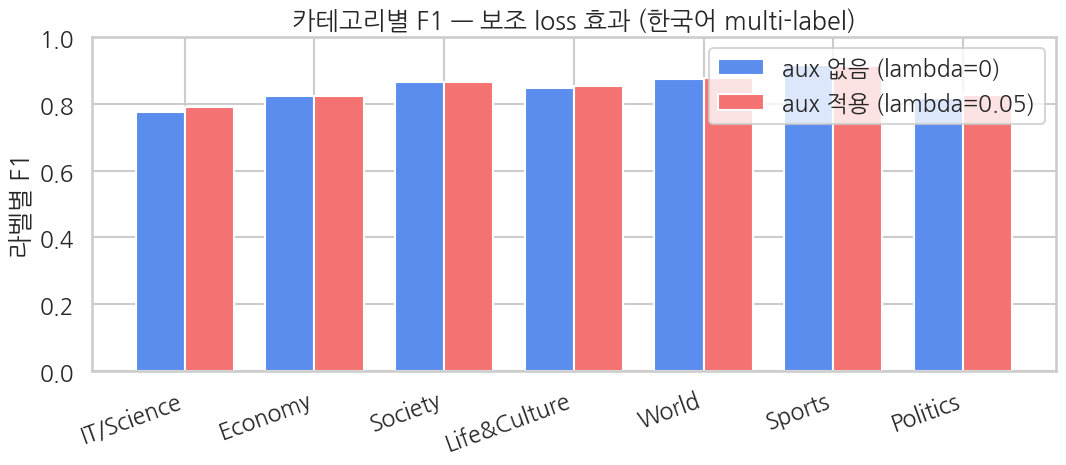
\includegraphics[width=0.88\linewidth]{assets/figures/ch18_per_label_f1_compare.png}
\end{bookfigurelabel}

\textbf{그림 읽기} --- 그림~\ref{fig:ch18-per-label-f1-compare}에서 다음 내용을 확인합니다: 한국어 보조 손실 적용 전후의 카테고리별 F1 비교. 실행된 노트북에서 저장된 최신 plot 출력이므로, 코드에서 계산한 값이 어떤 평가 지점으로 이어지는지 바로 확인할 수 있습니다.



\textbf{해석}

\begin{itemize}
\tightlist
\item
  \textbf{활성률 높은 카테고리} (스포츠/세계/사회 등): baseline 자체 F1 이 높음. delta 는 작거나 0 --- 이미 신호가 충분.
\item
  \textbf{활성률 낮은·혼동하는 카테고리} (정치/IT과학 등): baseline F1 이 낮음. 보조 신호의 \emph{정규화 효과} 가 상대적으로 도움이 될 가능성 --- 그래도 5K 샘플·2 epoch quick 모드에선 delta 가 노이즈 영역 (±0.01) 안에 머무를 수 있음.
\item
  \textbf{모든 카테고리 delta 가 ±0.005 이내} \(\to\) quick 모드 표본의 노이즈 영역. 학습량 (epoch·데이터) 을 늘려야 보조 효과가 통계적으로 분리 가능.
\end{itemize}



\subsection{보조 태스크 평가}

\inlinecode{n\_active} 는 1 또는 2 정수만 나오므로 \emph{binary 같은 회귀} 입니다. RMSE 가 0 에 가까우면 모델이 두 경우를 잘 구분, 0.5 근처면 무작위 추측 (분산이 0.25 인 1-vs-2 분포).



\Needspace{11\baselineskip}
\begin{lstlisting}
df_aux = pd.DataFrame({
    "실제 n_active": [f"{int(v)}" for v in aux_true],
    "예측값":     aux_preds_aux,
})
order = ["1", "2"]

fig, ax = plt.subplots(figsize=(7.5, 5.5))
sns.violinplot(
    data=df_aux, x="실제 n_active", y="예측값",
    order=order, inner="quart", cut=0,
    color="#F47272", alpha=0.6, ax=ax,
)

\end{lstlisting}

\noindent\emph{앞뒤 블록은 모두 숫자 결과를 그림으로 확인하는 단계입니다. 길이를 나누어 같은 흐름을 단계별로 확인합니다.}

\Needspace{11\baselineskip}
\begin{lstlisting}[firstnumber=14]
for i, target in enumerate([1.0, 2.0]):
    ax.hlines(
        target,
        i - 0.4,
        i + 0.4,
        color="black",
        lw=1.1,
        ls="--",
        alpha=0.7,
    )
ax.set_ylim(0.0, 3.0)
ax.set_title(f"보조 task — 예측 n_active vs 실제 n_active  (RMSE={rmse_aux:.3f}, r={pear_aux:.3f})")
plt.tight_layout()
plt.show()
\end{lstlisting}

\begin{bookfigurelabel}[H]{활성 라벨 개수 보조 회귀의 예측 분포}{fig:ch18-aux-count-violin}
\centering
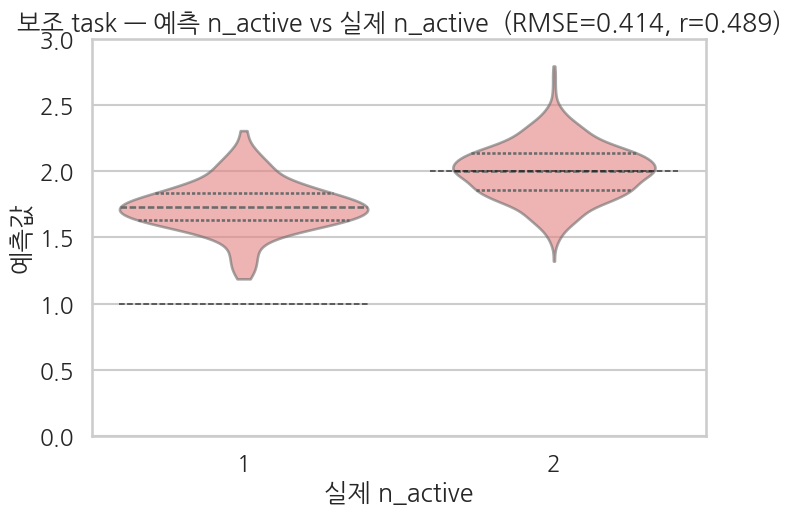
\includegraphics[width=0.76\linewidth]{assets/figures/ch18_aux_count_violin.png}
\end{bookfigurelabel}

\textbf{그림 읽기} --- 그림~\ref{fig:ch18-aux-count-violin}에서 다음 내용을 확인합니다: 활성 라벨 개수 보조 회귀의 예측 분포. 실행된 노트북에서 저장된 최신 plot 출력이므로, 코드에서 계산한 값이 어떤 평가 지점으로 이어지는지 바로 확인할 수 있습니다.



\textbf{해석}

\begin{itemize}
\tightlist
\item
  두 violin (n\_active=1, n\_active=2) 의 \emph{중심} 이 점선 가이드 (1.0 / 2.0) 에 잘 맞으면 보조 헤드가 활성 개수를 잘 학습한 것.
\item
  \emph{분포 폭} --- 모델이 두 경우를 \emph{자신 있게} 구분하면 violin 이 좁고 점선 가이드에 집중. 폭이 넓고 두 violin 이 0.5 근처에서 겹치면 학습 부족.
\item
  1.5 근처에 한 데가 몰려 있으면 \emph{상수 평균 예측} 으로 회귀 --- 보조 신호가 메인 표상에 \emph{반영되지 못한} 상태. 이 경우 \(\lambda\) 를 더 키우거나 데이터·epoch 를 늘려야 함.
\end{itemize}



\section{\texorpdfstring{변형: \(\lambda\) 스윕 (전체 곡선은 부록에서)}{변형: \textbackslash lambda 스윕 (전체 곡선은 부록에서)}}

§8 은 \(\lambda\)=0 vs \(\lambda\)=0.05 \emph{두 점} 만 비교했습니다. \textbf{\(\lambda\) 전체 곡선(0 \(\to\) 0.5)은 부록 \inlinecode{18\_ko\_auxiliary\_lambda\_sweep} 에서 실측} 으로 그립니다 --- sweet spot 이 \(\lambda\)=0.05 이고, \(\lambda\)\(\ge\)0.2 부터 메인이 무너지는 모습, 그리고 \ref{ch:14}장(강한 보조)와의 대조를 거기서 봅니다.

아래는 이 노트북 안에서 \emph{빠르게} 몇 점만 직접 돌려보고 싶을 때의 선택 코드입니다 (각 \(\lambda\) 마다 처음부터 재학습 --- 시간 여유 있을 때만).



\Needspace{11\baselineskip}
\begin{lstlisting}
LAMBDA_GRID = [0.0, 0.1, 1.0]
RUN_LAMBDA_SWEEP = False

sweep_results = []

if RUN_LAMBDA_SWEEP:
    for lam in LAMBDA_GRID:
        print(f"\n{'='*60}")
        print(f"Training with lambda_aux = {lam}")
        print(f"{'='*60}")
        m = make_model()
        args = TrainingArguments(
            output_dir=f"./ch18_sweep_lam{lam}",
            num_train_epochs=2,
            per_device_train_batch_size=16,
            per_device_eval_batch_size=32,
\end{lstlisting}

\noindent\emph{앞 블록은 학습 설정을 만들고 학습 루프를 실행하는 단계입니다. 이어지는 블록에서는 텍스트를 모델 입력 텐서로 바꾸는 단계로 넘어갑니다.}

\Needspace{11\baselineskip}
\begin{lstlisting}[firstnumber=17]
            learning_rate=2e-5,
            fp16=True,
            eval_strategy="no",
            logging_steps=200,
            save_strategy="no",
            report_to="none",
            seed=SEED,
            remove_unused_columns=False,
        )
        tr = AuxTrainer(
            model=m, args=args,
            train_dataset=train_tok, eval_dataset=eval_tok,
            data_collator=collator, processing_class=tokenizer,
            compute_metrics=compute_metrics_main, lambda_aux=lam,
        )
        tr.train()
\end{lstlisting}

\noindent\emph{앞 블록은 텍스트를 모델 입력 텐서로 바꾸는 단계입니다. 이어지는 블록에서는 앞에서 만든 중간 값을 다음 계산으로 넘기는 단계로 넘어갑니다.}

\Needspace{11\baselineskip}
\begin{lstlisting}[firstnumber=33]
        ev = tr.evaluate()
        sweep_results.append({
            "lambda": lam,
            "macro_f1": float(ev.get("eval_macro_f1", float("nan"))),
            "micro_f1": float(ev.get("eval_micro_f1", float("nan"))),
            "macro_auc": float(ev.get("eval_macro_auc", float("nan"))),
        })
        del m, tr
        if torch.cuda.is_available():
            torch.cuda.empty_cache()

\end{lstlisting}

\noindent\emph{앞뒤 블록은 모두 앞에서 만든 중간 값을 다음 계산으로 넘기는 단계입니다. 길이를 나누어 같은 흐름을 단계별로 확인합니다.}

\Needspace{10\baselineskip}
\begin{lstlisting}[firstnumber=44]
    sweep_df = pd.DataFrame(sweep_results)
    print("\nLambda sweep result:")
    print(sweep_df.round(4).to_string(index=False))
else:
    print(
        "Lambda sweep skipped. Set RUN_LAMBDA_SWEEP=True "
        "to run (~30 min extra on T4)."
    )
\end{lstlisting}

\noindent\textbf{출력.}
\begin{bookoutputbox}
Lambda sweep skipped. Set RUN_LAMBDA_SWEEP=True to run (~30 min extra on T4).
\end{bookoutputbox}
\par\vspace{0.9em}



\textbf{해석 가이드 --- 결과를 직접 보면}

\begin{itemize}
\tightlist
\item
  macro\_f1 이 \(\lambda\)=0.1 에서 최대 \(\to\) 간단한 보조 가중치가 정규화 효과로 메인 도움.
\item
  macro\_f1 이 \(\lambda\)=1.0 에서 최대 \(\to\) 보조 신호가 충분히 강해 둘 다 학습.
\item
  macro\_f1 이 \(\lambda\)=0 에서 최대 (baseline 이 가장 좋음) \(\to\) 보조 task 가 이 셋업에선 도움 안 됨. quick 모드 노이즈일 수 있어 시드 바꿔 재실행 권장.
\end{itemize}



\section{결과 해석 --- sweet spot 에서는 약한 보조도 메인을 (살짝) 돕는다}

§8 비교에서 \textbf{\(\lambda\)=0.05 보조가 \(\lambda\)=0 baseline 을 micro·macro-F1 모두에서 앞섰습니다} (각 +0.003, +0.004). \inlinecode{n\_active} 라는 \emph{약한} 보조 신호도 작은 \(\lambda\) 에서는 공유 KLUE-BERT 본체에 간단한 정규화로 작용해 메인 분류를 살짝 끌어올립니다.

다만 그 효과는 \textbf{\ref{ch:14}장(영어, 별점 보조)보다 작습니다.} 부록 \inlinecode{18\_ko\_auxiliary\_lambda\_sweep} 의 \(\lambda\) 곡선과 \ref{ch:14}장 를 나란히 두면:

\begin{booktable}{18장 결과 해석 - sweet spot 에서는 약한 보조도 메인을 (살짝) 돕는다 표}{tab:ch18-05}
\begin{adjustbox}{max width=\textwidth}
\begin{tabular}{@{}llll@{}}
\toprule
& 보조 task & 보조 R² & sweet spot \(\Delta\)(micro) \\
\midrule

\ref{ch:14}장 & 별점 회귀 & 0.43 (강함) & +0.007 \\
\textbf{\ref{ch:18}장} & \textbf{n\_active 회귀} & \textbf{0.065 (약함)} & \textbf{+0.003} \\
\bottomrule
\end{tabular}
\end{adjustbox}
\end{booktable}

두 장의 sweet spot 은 똑같이 \textbf{\(\lambda\)=0.05} 인데 도움의 \emph{크기} 가 다릅니다. 차이는 \(\lambda\) 가 아니라 \textbf{보조 신호의 정보량} 입니다.

\subsection{\texorpdfstring{왜 \inlinecode{n\_active} 는 약한가}{왜 n\_active 는 약한가}}

\inlinecode{n\_active} 는 합성 규칙상 거의 항상 2 입니다 (train 분포 \{1: 732, 2: 4268\}). 분산이 작아 \emph{예측할 게 별로 없어서}, 보조 헤드가 \(\lambda\) 를 0.5 까지 키워도 R² 가 0.08 에 머뭅니다. 보조가 입력을 깊이 들여다볼 동기가 약하니 공유 표현에 실어주는 추가 정보도 적습니다. 반면 \ref{ch:14}장의 별점은 \emph{사용자가 직접 매긴} 입력 의존도 높은 신호라 R² 0.43 으로 잘 학습되고, 그만큼 메인에도 더 보탬이 됐습니다.

\subsection{\texorpdfstring{\(\lambda\) 를 키우면}{\textbackslash lambda 를 키우면}}

\(\lambda\)\(\ge\)0.2 부터는 약한 보조가 오히려 메인을 깎습니다 (\(\lambda\)=0.5 에서 micro 0.80). 약한 보조일수록 \emph{도움이 되는 작은 \(\lambda\) 구간이 더 좁습니다} --- 본편이 \(\lambda\)=0.05 를 쓰는 이유입니다.

\begin{quote}
\emph{이 장의 메시지} --- auxiliary loss 는 공짜 만병통치약이 아니라, \textbf{(1) \(\lambda\) 를 작게 잡고 (2) 입력 의존도 높은 보조 신호를 골라야} 메인을 돕습니다. \inlinecode{n\_active} 는 데이터 합성의 자연 부산물이라 손쉽지만 약하고, 그래도 sweet spot 에서는 +가 납니다. 더 큰 도움을 원하면 헤드라인 길이·발행 메타데이터처럼 \emph{입력 의존도 큰} 보조로 바꾸는 게 다음 수입니다.
\end{quote}



\section{이 장에 등장한 라이브러리·함수}

\begin{booktable}{18장 새로 등장한 라이브러리}{tab:ch18-06}
\begin{adjustbox}{max width=\textwidth}
\begin{tabular}{@{}lll@{}}
\toprule
이름 & 한 줄 설명 & 다음 장에서 \\
\midrule

\inlinecode{AutoModel.from\_pretrained(...)} & 분류 헤드 없이 BERT 본체만 로드 --- 메인·보조 헤드를 직접 부착 & Phase 3 토크나이저 학습엔 등장 안 함 (\ref{ch:19}장 부터는 본체보다 어휘 자체에 집중) \\
커스텀 \inlinecode{nn.Module} (KoBertMultiTask) & 본체 공유 + 두 헤드 명시 정의 --- multi-task 정통 패턴 & GPT 장 (\ref{ch:21}장) 의 task-specific head 패턴과 연결 \\
\inlinecode{Trainer.compute\_loss} 오버라이드 + \inlinecode{lambda\_aux} 인자 & 자동 매핑이 못 다루는 \emph{복합 loss} + \(\lambda\) 동적 주입 & \(\lambda\) grid search 패턴 \\
커스텀 \inlinecode{AuxCollator} & input\_ids 외 \emph{추가 라벨} (n\_active) 도 batch 에 같이 담기 & \ref{ch:14}장과 같은 패턴, 보조 신호 변형마다 재사용 \\
\inlinecode{remove\_unused\_columns=False} & 모델 시그니처와 무관하게 모든 컬럼 통과 & custom collator 패턴마다 \\
\inlinecode{SequenceClassifierOutput} & Trainer 호환 출력 형식 (loss + logits) --- 커스텀 모델에서도 표준 dict 반환 & 커스텀 모델 패턴마다 \\
\inlinecode{r2\_score}, \inlinecode{np.corrcoef} & 회귀 보조 metric (R², Pearson r) & 회귀 결합 task 마다 \\
\bottomrule
\end{tabular}
\end{adjustbox}
\end{booktable}



\section{체크포인트 질문}

\begin{enumerate}
\def\labelenumi{\arabic{enumi}.}
\tightlist
\item
  \ref{ch:14}장 (영어 별점 보조) 와 \ref{ch:18}장 (한국어 활성 개수 보조) 의 \emph{변경된 축} 은 무엇인가요? \emph{한 가지 축} 원칙 관점에서 어느 쪽이 더 “loss 축 변화” 에 가까운가요?
\item
  \inlinecode{n\_active} 가 메인 multi-hot 벡터의 \emph{합} 이라는 점이 보조 task 로서 \emph{유리한 점} 과 \emph{불리한 점} 을 각각 한 줄로.
\item
  \inlinecode{AutoModelForSequenceClassification} 대신 \inlinecode{AutoModel\ +\ 커스텀\ nn.Module} 로 간 이유는? 어떤 상황에서 자동 매핑이 부족한가요?
\item
  \(\lambda\)=0.1 을 기본값으로 잡은 근거는? (메인 BCE 와 보조 MSE 의 \emph{크기 자체} 가 어떻게 다른가)
\end{enumerate}



\section{FAQ}

\begin{faqBox}{Q1. (실무) \inlinecode{n\_active} 외에 어떤 보조 task 를 시도할 수 있나요?}

KLUE-YNAT 합성 데이터에서 \emph{공짜로} 얻을 수 있는 보조 신호:

\begin{booktable}{18장 FAQ 표}{tab:ch18-07}
\begin{adjustbox}{max width=\textwidth}
\begin{tabular}{@{}lll@{}}
\toprule
보조 task & 라벨 형식 & 예상 효과 \\
\midrule

헤드라인 길이 (토큰 수) & float (정규화) & 약함 --- 길이는 카테고리와 상관 약함 \\
두 원본 헤드라인의 \emph{주제 유사도} & float {[}0, 1{]} & 중간 --- 유사 주제 결합 vs 이질 결합 구분 \\
두 카테고리의 \emph{id 차이} \inlinecode{abs(c\_A\ -\ c\_B)} & int & 약함 --- id 자체가 의미 없음 \\
\textbf{원본 단일 카테고리 예측} (combined 가 아닌 \emph{각 절반} 의 카테고리) & int & 강함 --- 메인과 직접 관련, 추천 \\
\bottomrule
\end{tabular}
\end{adjustbox}
\end{booktable}

원본 카테고리 예측을 보조로 쓰려면 \inlinecode{make\_multilabel} 에서 \inlinecode{(c\_A,\ c\_B)} 를 \emph{순서 라벨} 로 보존하고 보조 헤드를 \texttt{Linear(H,\ K)\ \$\textbackslash{}times\$\ 2} 로 두 개 만들면 됩니다 (multi-task 가 \emph{3-task} 가 됨 --- multi-label + 2개 single-label).

\end{faqBox}

\begin{faqBox}{Q2. (이론) \inlinecode{n\_active} 가 메인의 \emph{합} 이라는 게 왜 \emph{보조로 쓰면 의외로 약한} 신호인가요?}

직관적으로는 “메인을 잘 풀면 합도 잘 풂” 인데, 역방향 (“합을 잘 풀면 메인도 잘 풂”) 의 정보량이 작기 때문입니다.

\begin{itemize}
\tightlist
\item
  메인이 잘 풀린 모델 \(\to\) \inlinecode{n\_active} 도 잘 추정 (정의상 합이니까).
\item
  그러나 \emph{보조만 잘 학습} 된 모델 \(\to\) “이 헤드라인이 1개 vs 2개 카테고리에 걸친다” 만 알지 \emph{어느} 카테고리인지의 정보는 없음. 표현 공간이 카테고리 \emph{식별} 방향이 아니라 \emph{개수} 방향으로 발전.
\item
  BCE per-label 의 gradient 가 \emph{어느} 카테고리를 활성할지 직접 학습 신호. MSE on n\_active 의 gradient 는 \emph{몇 개} 인지만 학습 신호.
\end{itemize}

따라서 \inlinecode{n\_active} 가 메인의 \emph{함수} 이긴 하지만 \emph{전사 가능한 inverse 가 없는 함수} 라 보조로서의 추가 정보량이 제한적. \ref{ch:14}장의 별점은 항목 분류와 \emph{부분} 상관이지만 \emph{완전히 다른 방향} 의 정보 (감성) 라 BERT 표상에 \emph{추가} 차원을 만듭니다 --- 그래서 보조 효과 자체는 별점 쪽이 클 가능성.

\end{faqBox}

\begin{faqBox}{Q3. (실무) \inlinecode{AutoModel\ +\ nn.Module} 패턴이 \inlinecode{model.aux\_head\ =\ nn.Linear(...)} 한 줄 부착보다 권장되는 경우는?}

\begin{booktable}{18장 FAQ 표}{tab:ch18-08}
\begin{adjustbox}{max width=\textwidth}
\begin{tabular}{@{}ll@{}}
\toprule
상황 & 권장 패턴 \\
\midrule

보조 헤드 1개, 메인은 표준 분류 & 한 줄 부착 (\ref{ch:14}장 패턴) --- 간결 \\
보조 헤드 2개+, 또는 메인 헤드도 비표준 & \inlinecode{nn.Module} 정의 (\ref{ch:18}장 패턴) --- 명시성 \\
layer-wise lr 차등 (BERT 본체는 작은 lr, 헤드는 큰 lr) & \inlinecode{nn.Module} --- \inlinecode{named\_parameters} 로 그룹 분리 쉬움 \\
헤드별 dropout 등 미세 조정 & \inlinecode{nn.Module} --- \inlinecode{\_\_init\_\_} 에서 한 곳에 정의 \\
BERT 본체 일부 layer freeze & 둘 다 가능, 명시 정의가 가독성 더 좋음 \\
\bottomrule
\end{tabular}
\end{adjustbox}
\end{booktable}

\Needspace{8\baselineskip}
\begin{lstlisting}
optimizer_grouped = [
    {"params": [p for n, p in model.named_parameters() if n.startswith("bert.")],   "lr": 2e-5},
    {"params": [p for n, p in model.named_parameters() if n.startswith("cls_head")],"lr": 1e-4},
    {"params": [p for n, p in model.named_parameters() if n.startswith("count_head")],"lr": 1e-4},
]
optimizer = torch.optim.AdamW(optimizer_grouped)
\end{lstlisting}

\end{faqBox}

\begin{faqBox}{Q4. (이론) 보조 loss 가 \emph{MSE} 대신 \emph{MAE (L1)} 면 학습 양상이 어떻게 달라지나요?}

\inlinecode{n\_active} 는 1 또는 2 정수라 분포가 \emph{binary 같음}. MAE 와 MSE 의 차이:

\begin{itemize}
\tightlist
\item
  \textbf{MSE}: gradient 가 잔차에 \emph{비례} --- 큰 오차에 큰 gradient. 평균값 (\(\sim\) 1.86) 으로 수렴.
\item
  \textbf{MAE (L1)}: gradient 가 잔차의 \emph{부호} 만 (크기 일정 ±1). 중앙값 (= 2, 빈도 6/7) 으로 수렴.
\end{itemize}

따라서 MAE 로 바꾸면 보조 헤드가 \emph{항상 2 를 예측} 하게 되어 (중앙값 = 2) 학습 신호가 거의 없습니다. binary-같은 회귀에선 MSE 가 더 적절.

또 다른 선택: \inlinecode{n\_active\ -\ 1} 을 \emph{binary 분류} 로 풀어 \inlinecode{BCEWithLogitsLoss} 적용 --- 1 vs 2 를 0 vs 1 로 매핑. 회귀보다 분류가 더 자연스러운 형식이지만, \emph{연속적 보조 신호} 라는 multi-task 의 전통적 셋업에선 회귀가 일반적.

\Needspace{9\baselineskip}
\begin{lstlisting}
aux_logits = self.count_head(cls).squeeze(-1)   # (B,)
aux_target = (n_active - 1).float()
# 1$\to$0, 2$\to$1
l_aux = F.binary_cross_entropy_with_logits(
    aux_logits,
    aux_target,
)
\end{lstlisting}

\end{faqBox}

\begin{faqBox}{Q5. (실무) 학습 중 보조 loss 가 \emph{증가} 하면 어떻게 진단하나요?}

\inlinecode{logging\_steps=50} 으로 학습 곡선 (train loss) 만 보면 \emph{combined loss 만} 출력됩니다. 보조 loss 만 분리해 추적하려면 \inlinecode{compute\_loss} 안에서 직접 log:

\Needspace{11\baselineskip}
\begin{lstlisting}
def compute_loss(self, model, inputs, return_outputs=False, num_items_in_batch=None):
    inputs = {**inputs, "lambda_aux": self.lambda_aux}
    outputs = model(**inputs)
    loss = outputs.loss

    if self.state.global_step % 50 == 0 and not return_outputs:

        with torch.no_grad():
            cls = model.bert(**{k: v for k, v in inputs.items()
\end{lstlisting}

\noindent\emph{앞뒤 블록은 모두 앞에서 만든 중간 값을 다음 계산으로 넘기는 단계입니다. 길이를 나누어 같은 흐름을 단계별로 확인합니다.}

\Needspace{11\baselineskip}
\begin{lstlisting}[firstnumber=10]
                                if k in ("input_ids", "attention_mask", "token_type_ids")}
                            ).last_hidden_state[:, 0, :]
            count_pred = model.count_head(cls).squeeze(-1)
            l_aux_only = F.mse_loss(count_pred, inputs["n_active"].float()).item()
        print(
            f"step {self.state.global_step}  main+aux={loss.item():.4f}  aux_only="
            f"{l_aux_only:.4f}"
        )
    return (loss, outputs) if return_outputs else loss
\end{lstlisting}

보조 loss 가 \emph{상승} 한다면:

\begin{itemize}
\tightlist
\item
  \(\lambda\) 가 너무 작아 보조 학습이 \emph{메인 방향에 휘둘림} --- \(\lambda\) 키워 보조 학습 강화.
\item
  또는 메인과 보조가 \emph{충돌 방향} --- \(\lambda\) 줄이거나 보조 제거.
\end{itemize}

\end{faqBox}

\begin{faqBox}{Q6. (이론) \ref{ch:14}장과 \ref{ch:18}장의 결과 (delta) 패턴이 \emph{다를} 거라 예상되는 이유는?}

\begin{booktable}{18장 FAQ 표}{tab:ch18-09}
\begin{adjustbox}{max width=\textwidth}
\begin{tabular}{@{}lll@{}}
\toprule
측면 & \ref{ch:14}장 (영어, 별점) & \ref{ch:18}장 (한국어, n\_active) \\
\midrule

보조 신호의 \emph{입력 의존도} & 높음 --- 사용자가 \emph{직접} 매긴 감성 평가 & 낮음 --- 합성 규칙의 기계적 함수 (1/7 확률) \\
보조 신호의 \emph{메인과의 독립 차원} & 다른 차원 (감성 vs 항목) & 같은 차원의 함수 (합) \\
보조 정답의 분포 & 1-5 별점 (5 카테고리) & 1 또는 2 (이항 같음) \\
보조 정답 예측 난이도 & 중간 --- 진짜 회귀 & 매우 쉬움 --- 상수 평균만 예측해도 RMSE 작음 \\
예상 메인 delta & 약 양수 (별점 신호가 항목 표상 보강) & 약 0 (n\_active 신호가 추가 정보 적음) \\
\bottomrule
\end{tabular}
\end{adjustbox}
\end{booktable}

따라서 quick 모드에선 \ref{ch:18}장 delta 가 \emph{더 작게} 나올 가능성. 그래도 셋업 자체는 \emph{멀티태스크 학습의 정통 패턴} 을 한국어 환경에서 검증하는 가치가 있고, FAQ Q1 처럼 \emph{더 유용한 보조 task} 로 확장하는 출발점.

\end{faqBox}

\begin{faqBox}{Q7. (실무) Phase 2 (한국어, \ref{ch:15}--\ref{ch:18}장) 가 끝났습니다. Phase 3 에서 토크나이저를 \emph{직접 학습} 하는 이유는?}

\ref{ch:01}--\ref{ch:18}장 모두 \emph{사전학습 토크나이저} (sklearn TF-IDF 토큰화, BERT WordPiece) 에 의존했습니다. Phase 3 (\ref{ch:19}--\ref{ch:23}장) 는 이 의존을 끊고 \emph{어휘 자체를 코퍼스에서 학습}:

\begin{itemize}
\tightlist
\item
  \textbf{\ref{ch:19}장}: BPE / WordPiece / Unigram 알고리즘을 직접 돌려 어휘 만들기 \(\to\) 토큰화가 \emph{데이터에 따라 어떻게 달라지는지} 직관.
\item
  \textbf{\ref{ch:20}장}: 학습한 토크나이저로 \emph{작은 BERT 를 처음부터} 사전학습 \(\to\) 사전학습 의존 없는 경험.
\end{itemize}

\begin{quote}
Phase 3 가 클라이맥스인 이유 --- \ref{ch:01}장 부터 따라온 “ 토크나이저 노트” 가 \emph{외부 도구의 사용법} 이었다면 Phase 3 는 \emph{그 도구 자체를 만드는 단계}. 토크나이저를 직접 만들고 나면 \ref{ch:01}--\ref{ch:18}장의 모든 토큰화 노트를 \emph{다시 읽었을 때} 보이는 풍경이 달라집니다.
\end{quote}
\end{faqBox}



\section{오류 실험 (선택)}

다음 두 가지 흔한 함정:

\textbf{1. \inlinecode{remove\_unused\_columns=True} (기본값) 로 두기}

\Needspace{6\baselineskip}
\begin{lstlisting}
training_args = TrainingArguments(
    ...,
    remove_unused_columns=True,
)
\end{lstlisting}

Trainer 가 model.forward 시그니처를 검사해 \emph{맞지 않는 컬럼은 제거}. \inlinecode{n\_active} 가 시그니처에 있긴 하지만 자동 검사가 실패할 때 (e.g. 커스텀 모델 시그니처 변경 시) \inlinecode{n\_active} 가 사라져 \inlinecode{compute\_loss} 안에서 None 이 됩니다. 안전상 \inlinecode{False} 권장.

\textbf{2. \inlinecode{count\_pred} 를 모델 attribute 에 저장 안 하기}

\Needspace{5\baselineskip}
\begin{lstlisting}
return SequenceClassifierOutput(loss=loss, logits=main_logits)
\end{lstlisting}

\inlinecode{SequenceClassifierOutput} 은 \inlinecode{loss}/\inlinecode{logits}/\inlinecode{hidden\_states}/\inlinecode{attentions} 만 표준 필드. \inlinecode{count\_pred} 를 추가하려면 dataclass 를 직접 정의하거나, 본문처럼 \inlinecode{self.last\_count\_pred\ =\ ...} 에 저장해 eval 단계에서 꺼냅니다. 후자가 간단하지만 \emph{멀티 GPU 학습 시 race condition} 가능 --- 운영 코드는 정식 dataclass 정의 권장.



\begin{previewBox}{미리보기: 다음 장}

\textbf{\ref{ch:19}장. 토크나이저 직접 학습 --- BPE / WordPiece / Unigram}

\begin{itemize}
\tightlist
\item
  Phase 1-2 영어·한국어 모두 \emph{사전학습 토크나이저} 를 그대로 썼습니다. \ref{ch:19}장 는 그 의존을 끊고 \emph{어휘를 코퍼스에서 직접 학습}.
\item
  \inlinecode{tokenizers} 라이브러리로 BPE, WordPiece, Unigram 세 알고리즘을 같은 코퍼스에 적용해 \emph{어휘 차이} 비교.
\item
  한국어 vs 영어 코퍼스에서 학습한 토크나이저의 \emph{토큰 길이 분포} 가 어떻게 다른지 --- \ref{ch:01}장 부터 추적해 온 토크나이저 시각의 완성.
\end{itemize}

\begin{quote}
\textbf{Phase 2 마무리} --- \ref{ch:15}--\ref{ch:18}장 을 통해 한국어 BERT 의 binary·multi-class·multi-label·auxiliary 4 가지를 다 익혔습니다. Phase 3 는 한 발 더 내려가 \emph{어휘 구성} 자체에 도전 --- 사전학습 모델에 \emph{완전히 의존하지 않는} 경험.
\end{quote}

\begin{quote}
\textbf{변하는 축}: 모델·loss·task 가 아니라 \emph{토크나이저 그 자체} 가 학습 대상. 입력 표현이 만들어지는 \emph{가장 아래 단계} 로 내려갑니다.
\end{quote}
\end{previewBox}



\section{\texorpdfstring{부록: $\lambda$ 스윕: 약한 보조 task 의 sweet spot}{부록: lambda 스윕: 약한 보조 task 의 sweet spot}}



\Needspace{5\baselineskip}
\begin{lstlisting}
!pip install -q transformers datasets
\end{lstlisting}



\Needspace{10\baselineskip}
\begin{lstlisting}
import warnings; warnings.filterwarnings("ignore")
import numpy as np, pandas as pd
import matplotlib.pyplot as plt, seaborn as sns
import torch, torch.nn as nn, torch.nn.functional as F
from datasets import Dataset, load_dataset
from transformers import AutoTokenizer, AutoModel, Trainer, TrainingArguments, DataCollatorWithPadding
from transformers.modeling_outputs import SequenceClassifierOutput
from sklearn.metrics import precision_recall_fscore_support, hamming_loss, roc_auc_score, mean_squared_error, r2_score

\end{lstlisting}

\noindent\emph{앞뒤 블록은 모두 필요한 라이브러리와 기본 설정을 준비하는 단계입니다. 길이를 나누어 같은 흐름을 단계별로 확인합니다.}

\Needspace{11\baselineskip}
\begin{lstlisting}[firstnumber=10]
import matplotlib.pyplot as plt, matplotlib.font_manager as fm, subprocess, os
_fp = "/usr/share/fonts/truetype/nanum/NanumGothic.ttf"
if not os.path.exists(_fp):
    subprocess.run(
        "apt-get -qq -y install fonts-nanum",
        shell=True,
    )
fm.fontManager.addfont(_fp)
plt.rcParams["font.family"] = "NanumGothic"
plt.rcParams["axes.unicode_minus"] = False
print(
    f"PyTorch: {torch.__version__}  CUDA: "
    f"{torch.cuda.is_available()}"
)
if torch.cuda.is_available(): print(f"GPU: {torch.cuda.get_device_name(0)}")
\end{lstlisting}

\noindent\textbf{출력.}
\begin{bookoutputbox}
PyTorch: 2.11.0+cu128  CUDA: True
GPU: Tesla T4
\end{bookoutputbox}
\par\vspace{0.9em}



\subsection{데이터·모델·Trainer --- 본편 \ref{ch:18}장과 동일}

KLUE-YNAT 두 헤드라인을 결합한 합성 multi-label(7) + 활성 개수 \inlinecode{n\_active} 보조. \inlinecode{KoBertMultiTask}(AutoModel 본체 + 메인 헤드 + 보조 헤드) forward 안에서 \texttt{L\_main\ +\ \$\textbackslash{}lambda\$·L\_aux} 계산.



\Needspace{11\baselineskip}
\begin{lstlisting}
SEED = 42; N_TRAIN = 5000; N_EVAL = 1000
ds = load_dataset("klue/klue", "ynat").rename_column("title", "text")
K = len(ds["train"].features["label"].names)

def make_multilabel(source_split, n_samples, seed):
    rng = np.random.default_rng(seed); n_src = len(source_split)
    idx = rng.integers(0, n_src, size=2 * n_samples).tolist()
    idx_a, idx_b = idx[:n_samples], idx[n_samples:]
    src_text = list(source_split["text"]); src_label = list(source_split["label"])
    texts, mhs, counts = [], [], []
    for a, b in zip(idx_a, idx_b):
        ca, cb = int(src_label[a]), int(src_label[b])
        mh = [0.0]*K; mh[ca] = 1.0; mh[cb] = 1.0
        texts.append(f"{src_text[a]} [SEP] {src_text[b]}"); mhs.append(mh); counts.append(int(sum(mh)))
    return Dataset.from_dict({"text": texts, "multi_hot": mhs, "n_active": counts})

\end{lstlisting}

\noindent\emph{앞 블록은 데이터를 불러오고 학습에 맞는 형태로 정리하는 단계입니다. 이어지는 블록에서는 텍스트를 모델 입력 텐서로 바꾸는 단계로 넘어갑니다.}

\Needspace{11\baselineskip}
\begin{lstlisting}[firstnumber=17]
train_full = make_multilabel(
    ds["train"],
    N_TRAIN,
    seed=SEED,
)
eval_full  = make_multilabel(
    ds["validation"],
    N_EVAL,
    seed=SEED + 1,
)
tokenizer = AutoTokenizer.from_pretrained("klue/bert-base")

\end{lstlisting}

\noindent\emph{앞뒤 블록은 모두 텍스트를 모델 입력 텐서로 바꾸는 단계입니다. 길이를 나누어 같은 흐름을 단계별로 확인합니다.}

\Needspace{11\baselineskip}
\begin{lstlisting}[firstnumber=29]
def tokenize_fn(batch):
    out = tokenizer(
        batch["text"],
        truncation=True,
        max_length=128,
    )
    out["labels"]   = [list(map(float, mh)) for mh in batch["multi_hot"]]
    out["n_active"] = [float(n) for n in batch["n_active"]]
    return out
keep = (
    "input_ids",
    "attention_mask",
    "token_type_ids",
    "labels",
    "n_active",
)
\end{lstlisting}

\noindent\emph{앞 블록은 텍스트를 모델 입력 텐서로 바꾸는 단계입니다. 이어지는 블록에서는 필요한 라이브러리와 기본 설정을 준비하는 단계로 넘어갑니다.}

\Needspace{11\baselineskip}
\begin{lstlisting}[firstnumber=45]
train_tok = train_full.map(tokenize_fn, batched=True).remove_columns([c for c in train_full.column_names if c not in keep])
eval_tok  = eval_full.map(tokenize_fn, batched=True).remove_columns([c for c in eval_full.column_names if c not in keep])

import collections
dist = collections.Counter(train_full["n_active"])
print(
    f"K={K}, train={len(train_tok)}, eval="
    f"{len(eval_tok)}"
)
print(
    "n_active 분포(train):", dict(sorted(dist.items())), "
    ""-> 거의 2 (두 문서 결합), 분산 작음"
)
\end{lstlisting}

\noindent\textbf{출력.}
\begin{bookoutputbox}
K=7, train=5000, eval=1000
n_active 분포(train): {1: 732, 2: 4268} -> 거의 2 (두 문서 결합), 분산 작음
\end{bookoutputbox}
\par\vspace{0.9em}



\Needspace{11\baselineskip}
\begin{lstlisting}
class AuxCollator:
    def __init__(
        self,
        tokenizer): self.base = DataCollatorWithPadding(tokenizer,
    )
    def __call__(self, features):
        n_act = torch.tensor(
            [f.pop("n_active") for f in features],
            dtype=torch.float,
        )
        batch = self.base(features); batch["labels"] = batch["labels"].float(); batch["n_active"] = n_act
        return batch
collator = AuxCollator(tokenizer)

\end{lstlisting}

\noindent\emph{앞 블록은 텍스트를 모델 입력 텐서로 바꾸는 단계입니다. 이어지는 블록에서는 모델 출력을 확률이나 예측값으로 바꾸는 단계로 넘어갑니다.}

\Needspace{11\baselineskip}
\begin{lstlisting}[firstnumber=15]
class KoBertMultiTask(nn.Module):
    def __init__(self, model_name="klue/bert-base", num_labels=7):
        super().__init__()
        self.num_labels = num_labels
        self.bert = AutoModel.from_pretrained(model_name)
        H = self.bert.config.hidden_size
        self.cls_head = nn.Linear(H, num_labels)
        self.count_head = nn.Linear(H, 1)
        self.config = self.bert.config
    def forward(self, input_ids=None, attention_mask=None, token_type_ids=None, labels=None, n_active=None, lambda_aux=0.1):
        kwargs = {"input_ids": input_ids, "attention_mask": attention_mask}
        if token_type_ids is not None: kwargs["token_type_ids"] = token_type_ids
        out = self.bert(**kwargs); cls = out.last_hidden_state[:, 0, :]
        main_logits = self.cls_head(cls); count_pred = self.count_head(cls).squeeze(-1)
        loss = None
\end{lstlisting}

\noindent\emph{앞뒤 블록은 모두 모델 출력을 확률이나 예측값으로 바꾸는 단계입니다. 길이를 나누어 같은 흐름을 단계별로 확인합니다.}

\Needspace{11\baselineskip}
\begin{lstlisting}[firstnumber=30]
        if labels is not None and n_active is not None:
            l_main = F.binary_cross_entropy_with_logits(
                main_logits,
                labels.float(),
            )
            l_aux  = F.mse_loss(
                count_pred,
                n_active.float(),
            )
            loss = l_main + lambda_aux * l_aux
        self.last_count_pred = count_pred.detach()
        return SequenceClassifierOutput(loss=loss, logits=main_logits)

def make_model(): return KoBertMultiTask("klue/bert-base", num_labels=K)

\end{lstlisting}

\noindent\emph{앞 블록은 모델 출력을 확률이나 예측값으로 바꾸는 단계입니다. 이어지는 블록에서는 학습 설정을 만들고 학습 루프를 실행하는 단계로 넘어갑니다.}

\Needspace{11\baselineskip}
\begin{lstlisting}[firstnumber=45]
class AuxTrainer(Trainer):
    def __init__(self, *args, lambda_aux=0.1, **kwargs):
        super().__init__(*args, **kwargs); self.lambda_aux = lambda_aux
    def compute_loss(self, model, inputs, return_outputs=False, num_items_in_batch=None):
        inputs = {**inputs, "lambda_aux": self.lambda_aux}
        outputs = model(**inputs); loss = outputs.loss
        return (loss, outputs) if return_outputs else loss

def compute_metrics_main(eval_pred):
    logits, labels = eval_pred
\end{lstlisting}

\noindent\emph{앞 블록은 학습 설정을 만들고 학습 루프를 실행하는 단계입니다. 이어지는 블록에서는 예측 결과를 지표와 표로 요약하는 단계로 넘어갑니다.}

\Needspace{11\baselineskip}
\begin{lstlisting}[firstnumber=55]
    if isinstance(logits, tuple): logits = logits[0]
    probs = 1.0/(1.0+np.exp(-logits)); preds = (probs >= 0.5).astype(int)
    _,_,f1_mi,_ = precision_recall_fscore_support(
        labels,
        preds,
        average="micro",
        zero_division=0,
    )
    _,_,f1_ma,_ = precision_recall_fscore_support(
        labels,
        preds,
        average="macro",
        zero_division=0,
    )
    return {"micro_f1": float(f1_mi), "macro_f1": float(f1_ma), "hamming_loss": float(hamming_loss(labels, preds))}

\end{lstlisting}

\noindent\emph{앞 블록은 예측 결과를 지표와 표로 요약하는 단계입니다. 이어지는 블록에서는 텍스트를 모델 입력 텐서로 바꾸는 단계로 넘어갑니다.}

\Needspace{11\baselineskip}
\begin{lstlisting}[firstnumber=71]
@torch.no_grad()
def aux_predictions(trainer, dataset, batch_size=64):
    trainer.model.eval(); device = trainer.model.bert.device; ap, at = [], []
    for i in range(0, len(dataset), batch_size):
        bf = [dict(dataset[j]) for j in range(i, min(i+batch_size, len(dataset)))]
        b = trainer.data_collator(bf); bod = {k: v.to(device) for k, v in b.items()}
        nat = bod.pop("n_active").cpu().numpy(); bod.pop("labels", None)
        _ = trainer.model(
            **bod,
            labels=None,
            n_active=None,
        )
        ap.extend(trainer.model.last_count_pred.cpu().numpy().tolist()); at.extend(nat.tolist())
    return np.array(ap), np.array(at)
print("setup 완료")
\end{lstlisting}

\noindent\textbf{출력.}
\begin{bookoutputbox}
setup 완료
\end{bookoutputbox}
\par\vspace{0.9em}



\subsection{\texorpdfstring{\(\lambda\) 스윕}{\textbackslash lambda 스윕}}

\texttt{\$\textbackslash{}lambda\$\ in\ \{0,\ 0.02,\ 0.05,\ 0.1,\ 0.2,\ 0.5\}} 각각 같은 초기화로 2 epoch 학습 \(\to\) 메인 micro/macro-F1 + 보조 R² 기록. \(\lambda\)=0.1 은 비교점입니다.



\Needspace{11\baselineskip}
\begin{lstlisting}
LAMBDAS = [0.0, 0.02, 0.05, 0.1, 0.2, 0.5]
rows = []
for lam in LAMBDAS:
    torch.manual_seed(42); np.random.seed(42)
    model = make_model()
    args = TrainingArguments(output_dir=f"./sweep_{lam}", num_train_epochs=2,
        per_device_train_batch_size=16, per_device_eval_batch_size=32, learning_rate=2e-5,
        fp16=True, eval_strategy="no", logging_steps=200, save_strategy="no",
        report_to="none", seed=42, remove_unused_columns=False)
    tr = AuxTrainer(model=model, args=args, train_dataset=train_tok, eval_dataset=eval_tok,
        data_collator=collator, processing_class=tokenizer, compute_metrics=compute_metrics_main, lambda_aux=lam)
    tr.train()
    mets = tr.evaluate(
        ); ap,
        at = aux_predictions(tr, eval_tok,
    )
\end{lstlisting}

\noindent\emph{앞 블록은 텍스트를 모델 입력 텐서로 바꾸는 단계입니다. 이어지는 블록에서는 앞에서 만든 중간 값을 다음 계산으로 넘기는 단계로 넘어갑니다.}

\Needspace{11\baselineskip}
\begin{lstlisting}[firstnumber=17]
    r2 = float(r2_score(at, ap))
    rows.append({"lambda": lam, "micro_f1": mets["eval_micro_f1"], "macro_f1": mets["eval_macro_f1"],
                 "hamming": mets["eval_hamming_loss"], "aux_r2": r2})
    print(
        f"lambda={lam:<5} micro-F1={mets['eval_micro_f1']:.4f}  macro-F1={mets['eval_macro_f1']:.4f}  aux_R2="
        f"{r2:+.3f}"
    )
    del model, tr; torch.cuda.empty_cache()
res = pd.DataFrame(rows)
print(); print(res.round(4).to_string(index=False))
\end{lstlisting}

\noindent\textbf{출력.}
\begin{bookoutputbox}
Key                                        | Status     |  | 
-------------------------------------------+------------+--+-

Step  Training Loss
----  -------------
200   0.334212
400   0.193545
600   0.159128
Train... Valid... Step Micro F1 Macro F1 Hammi... Runtime Sampl... Steps...
-------- -------- ---- -------- -------- -------- -------- -------- --------
0.159128 0.193365 626 0.849143 0.845101 0.075429 0.787400 1270.... 40.64...
lambda=0.0   micro-F1=0.8491  macro-F1=0.8451  aux_R2=-8.656
Key                                        | Status     |  | 
-------------------------------------------+------------+--+-

Step  Training Loss
...
\end{bookoutputbox}
\par\vspace{0.9em}



\subsection{\texorpdfstring{곡선 --- \(\lambda\) vs 메인 성능}{곡선 --- \textbackslash lambda vs 메인 성능}}



\Needspace{11\baselineskip}
\begin{lstlisting}
base_micro = float(res.loc[res["lambda"]==0.0, "micro_f1"].iloc[0])
base_macro = float(res.loc[res["lambda"]==0.0, "macro_f1"].iloc[0])
best_i = res["micro_f1"].idxmax(); best_lambda = float(res.loc[best_i, "lambda"]); best_micro = float(res.loc[best_i, "micro_f1"])
sns.set_theme(
    style="whitegrid",
    context="talk",
    font="NanumGothic",
    rc={"axes.unicode_minus": False},
)
fig, ax = plt.subplots(figsize=(9.5, 5.5))
\end{lstlisting}

\noindent\emph{앞 블록은 숫자 결과를 그림으로 확인하는 단계입니다. 이어지는 블록에서는 앞에서 만든 중간 값을 다음 계산으로 넘기는 단계로 넘어갑니다.}

\Needspace{11\baselineskip}
\begin{lstlisting}[firstnumber=11]
ax.plot(
    res["lambda"],
    res["micro_f1"],
    "o-",
    color="#5B8DEF",
    lw=2,
    label="micro-F1",
)
ax.plot(
    res["lambda"],
    res["macro_f1"],
    "s-",
    color="#F47272",
    lw=2,
    label="macro-F1",
)
\end{lstlisting}

\noindent\emph{앞뒤 블록은 모두 앞에서 만든 중간 값을 다음 계산으로 넘기는 단계입니다. 길이를 나누어 같은 흐름을 단계별로 확인합니다.}

\Needspace{11\baselineskip}
\begin{lstlisting}[firstnumber=27]
ax.axhline(
    base_micro,
    color="#5B8DEF",
    ls="--",
    alpha=0.5,
    label="micro baseline (lambda=0)",
)
ax.axhline(
    base_macro,
    color="#F47272",
    ls="--",
    alpha=0.5,
    label="macro baseline (lambda=0)",
)
\end{lstlisting}

\noindent\emph{앞뒤 블록은 모두 앞에서 만든 중간 값을 다음 계산으로 넘기는 단계입니다. 길이를 나누어 같은 흐름을 단계별로 확인합니다.}

\Needspace{11\baselineskip}
\begin{lstlisting}[firstnumber=41]
ax.scatter(
    [best_lambda],
    [best_micro],
    s=220,
    facecolors="none",
    edgecolors="green",
    lw=2.5,
    zorder=5,
    label=f"best lambda={best_lambda}",
)
ax.set_xlabel("lambda (보조 손실 가중치)"); ax.set_ylabel("메인 task F1")
ax.set_title("lambda 에 따른 메인 multi-label 성능 (한국어, 약한 보조)")
\end{lstlisting}

\noindent\emph{앞 블록은 앞에서 만든 중간 값을 다음 계산으로 넘기는 단계입니다. 이어지는 블록에서는 숫자 결과를 그림으로 확인하는 단계로 넘어갑니다.}

\Needspace{11\baselineskip}
\begin{lstlisting}[firstnumber=53]
ax.legend(
    fontsize=10,
    loc="lower left",
)
plt.tight_layout()
plt.show()

print(
    f"baseline(lambda=0): micro={base_micro:.4f} macro="
    f"{base_macro:.4f}"
)
print(
    f"best lambda={best_lambda}: micro={best_micro:.4f} (delta="
    f"{best_micro-base_micro:+.4f})"
)
print(
    f"lambda=0.1 (비교점): micro="
    f"{float(res.loc[res['lambda']==0.1,'micro_f1'].iloc[0]):.4f}"
)
\end{lstlisting}

\noindent\textbf{출력.}
\begin{bookoutputbox}
baseline(lambda=0): micro=0.8491 macro=0.8451
best lambda=0.05: micro=0.8523 (delta=+0.0032)
lambda=0.1 (비교점): micro=0.8489
\end{bookoutputbox}
\par\vspace{0.9em}

\begin{bookfigurelabel}[H]{한국어 보조 손실 lambda 스윕에서 확인한 sweet spot}{fig:ch18-lambda-sweep}
\centering
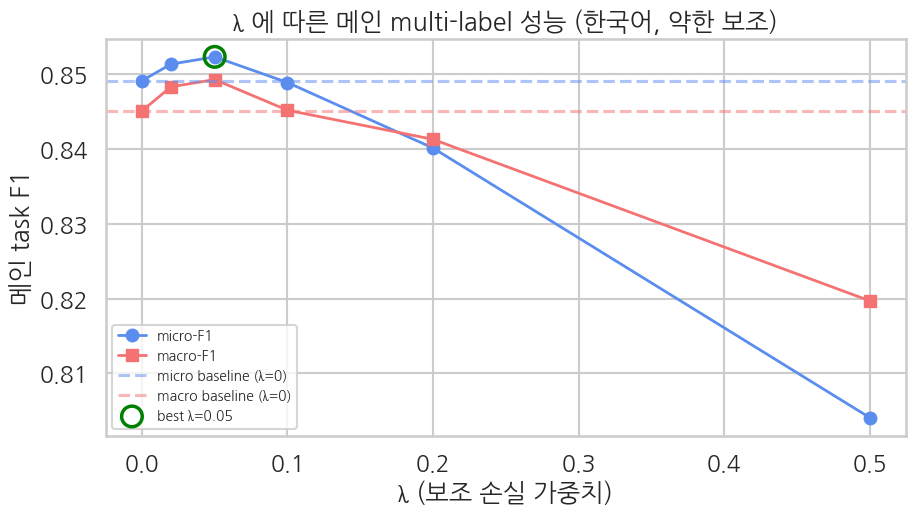
\includegraphics[width=0.86\linewidth]{assets/figures/ch18_lambda_sweep.png}
\end{bookfigurelabel}

\textbf{그림 읽기} --- 그림~\ref{fig:ch18-lambda-sweep}에서 다음 내용을 확인합니다: 한국어 보조 손실 lambda 스윕에서 확인한 sweet spot. 실행된 노트북에서 저장된 최신 plot 출력이므로, 코드에서 계산한 값이 어떤 평가 지점으로 이어지는지 바로 확인할 수 있습니다.



\subsection{해석}

\textbf{\(\lambda\)=0.05 가 sweet spot 입니다.} 메인 micro-F1 이 baseline(\(\lambda\)=0, 0.8491)보다 \textbf{+0.003 오른 0.8523}, macro 도 0.8451 \(\to\) 0.8493(\textbf{+0.004}). \emph{약한 보조(n\_active)도 작은 \(\lambda\) 에서는 메인을 살짝 끌어올립니다.} \(\lambda\)=0.1 은 공정 비교(같은 seed 초기화)에선 거의 \textbf{중립}(0.8489 \(\approx\) baseline)인 비교점입니다. \(\lambda\)\(\ge\)0.2 부터는 메인이 무너집니다(\(\lambda\)=0.5 에서 0.804).

\begin{booktable}{18장 해석 표}{tab:ch18-10}
\begin{adjustbox}{max width=\textwidth}
\begin{tabular}{@{}llll@{}}
\toprule
\(\lambda\) & micro-F1 & macro-F1 & 보조 R² \\
\midrule

0.0 (baseline) & 0.8491 & 0.8451 & --- \\
0.02 & 0.8514 & 0.8483 & 0.034 \\
\textbf{0.05 (sweet spot)} & \textbf{0.8523} & \textbf{0.8493} & 0.065 \\
0.1 (비교점) & 0.8489 & 0.8452 & 0.067 \\
0.2 & 0.8401 & 0.8413 & 0.073 \\
0.5 & 0.8041 & 0.8197 & 0.081 \\
\bottomrule
\end{tabular}
\end{adjustbox}
\end{booktable}

\subsubsection{\ref{ch:14}장(강한 보조)와의 대조 --- 이게 핵심}

두 장 모두 sweet spot 은 \textbf{\(\lambda\)=0.05} 로 같지만, 보조가 주는 도움의 \emph{크기} 가 다릅니다:

\begin{booktable}{18장 해석 표}{tab:ch18-11}
\begin{adjustbox}{max width=\textwidth}
\begin{tabular}{@{}llll@{}}
\toprule
& 보조 task & 보조 R² & sweet spot \(\Delta\)(micro) \\
\midrule

\ref{ch:14}장 (영어) & 별점 회귀 & 0.43 (강함) & \textbf{+0.007} \\
\ref{ch:18}장 (한국어) & n\_active 회귀 & 0.065 (약함) & \textbf{+0.003} \\
\bottomrule
\end{tabular}
\end{adjustbox}
\end{booktable}

\inlinecode{n\_active} 는 합성 규칙상 거의 항상 2 (분포 \{1: 732, 2: 4268\})라 분산이 작아 \textbf{예측할 게 별로 없습니다} --- \(\lambda\) 를 0.5 까지 키워도 보조 R² 가 0.08 에 머뭅니다. 그래서 \textbf{보조가 주는 도움도 \ref{ch:14}장의 절반 수준}. 보조 손실의 가치는 \emph{\(\lambda\) 만이 아니라 보조 신호가 얼마나 정보적인가} 에 비례합니다.

\begin{quote}
본편 \ref{ch:18}장은 이 sweet spot(\(\lambda\)=0.05)을 메인 학습값으로 쓰고, n\_active 의 약한 신호가 \emph{왜} \ref{ch:14}장 보다 도움이 작은지 짚습니다.
\end{quote}